\documentclass[11pt,a4paper]{article}

\usepackage[utf8]{inputenc}
\usepackage[T1]{fontenc}
\usepackage{lmodern}
\usepackage[spanish,es-noshorthands,es-tabla]{babel}
\usepackage[margin=2.3cm]{geometry}
\usepackage{graphicx}
\usepackage{float}
\usepackage{array}
\usepackage{longtable}
\usepackage{enumitem}
\usepackage[table]{xcolor}
\usepackage[hidelinks]{hyperref}

\graphicspath{{diagramas/}}
\newcolumntype{P}[1]{>{\raggedright\arraybackslash}p{#1}}
\setlist{itemsep=2pt,topsep=4pt}
\definecolor{cabecera}{HTML}{E7F5FF}

\begin{document}
\sloppy

\begin{titlepage}
  \centering
  \IfFileExists{logo.png}{%
    
\includegraphics[width=6cm]{logo.png}%
  }{%
    \fbox{\parbox[c][4cm][c]{7cm}{\centering\large Pontificia Universidad Javeriana}}%
  }
  \vspace{1.5cm}

  {\Huge\bfseries Documento de diseño\par}
  \vspace{0.6cm}
  {\LARGE Módulo de Reconstrucción\par}
  \vspace{0.3cm}
  {\large Plataforma de Gestión de Desastres y Reconstrucción\par}
  \vspace{0.6cm}
  {\large Versión 1.2\par}
  \vfill
  {\large Carlos Daniel Guiza \quad Juan Felipe Rubiano \quad Samuel Gantiva\par}
  \vspace{0.4cm}
  {\large Arquitectura de Software (004185)\par}
  \vspace{0.2cm}
  {\large Profesor: César Bustacara Medina\par}
  \vspace{0.2cm}
  {\large Pontificia Universidad Javeriana\par}
  \vspace{0.4cm}
  {\large 18 de noviembre de 2026\par}
\end{titlepage}

% ---------------------------------------------------------------------------
\section*{Control de cambios}

{\small
\begin{longtable}{|P{1.2cm}|P{2.6cm}|P{10.8cm}|}
  \hline
  \rowcolor{cabecera}\textbf{Versión} & \textbf{Fecha} & \textbf{Cambios} \\ \hline
  \endfirsthead
  \hline
  \rowcolor{cabecera}\textbf{Versión} & \textbf{Fecha} & \textbf{Cambios} \\ \hline
  \endhead
  1.0 & Noviembre de 2026 & Versión entregada: reglas de negocio, casos de uso CU-01 a CU-11, entidades,
    estados, arquitectura limpia, vista lógica, decisiones y tecnologías del módulo. \\ \hline
  1.2 & 18 de noviembre de 2026 & Alineación con el SAD 1.2, el SRS 1.2, el ATAM 1.2 y el código de la
    rama \texttt{cierre-implementacion}. Control de versiones y tabla de trazabilidad RF-RC $\rightarrow$
    CU $\rightarrow$ AD $\rightarrow$ QA. Reglas numeradas RN-RC-01 a RN-RC-22. Casos de uso con ruta HTTP y
    evento; CU-12 nuevo para el reporte de SE-7 (EV-24). Diagramas en PlantUML con notación UML: contexto, casos
    de uso, clases, estados, componentes, dos secuencias y despliegue. Vista lógica con los nombres del código y
    sin el \texttt{HistorialController} ni las tres consolas, que no existen. Decisiones DM-01 a DM-11 ligadas al
    SAD. La justificación de tecnología remite a AD-50 a AD-65 del SAD 1.2. Despliegue, implementación y alcance
    reescritos según \texttt{despliegue/compose/docker-compose.yml}. Enmiendas aplicadas: E-01, E-04, E-07,
    E-09, E-10, E-19, E-20, E-28, E-36 y E-39. Cada atributo se presenta con su nombre y su medida única; las
    tecnologías, con los atributos que favorecen y la alternativa descartada; los casos de uso, con su precondición y
    sus excepciones; y las tácticas y los patrones, con su tipo. Se agregan series de identificadores, límites,
    enmiendas y referencias. \\ \hline
\end{longtable}
}

\tableofcontents
\newpage

% ---------------------------------------------------------------------------
\section{Descripción general}
\label{sec:general}

Este documento diseña el módulo de Reconstrucción de la plataforma. El módulo crea proyectos de reconstrucción a
partir de las evaluaciones de daño validadas. Asigna presupuesto, fuente de financiación, cronograma y responsable.
Hace seguimiento al avance y a los costos. Deja cada cambio en un historial de solo inserción para auditoría.

El documento parte de las reglas de negocio (sección~\ref{sec:reglas}). Con ellas se construyen los casos de uso
(sección~\ref{sec:cu}), las entidades (sección~\ref{sec:entidades}) y el diagrama de estados del proyecto
(sección~\ref{sec:estados}). La arquitectura se presenta con el modelo 4+1 \cite{kruchten} restringido
al módulo, y cada vista sigue las recomendaciones de ISO/IEC/IEEE 42010 \cite{iso42010} y de Clements et
al. \cite{clements}:

\begin{itemize}
  \item \textbf{Escenarios}: diagrama y especificación de casos de uso (sección~\ref{sec:cu}).
  \item \textbf{Vista lógica}: entidades, anillos de la arquitectura limpia y componentes
        (secciones~\ref{sec:entidades} y~\ref{sec:logica}).
  \item \textbf{Vista de procesos}: colas y secuencias de CU-02 y CU-06 (sección~\ref{sec:procesos}).
  \item \textbf{Vista de desarrollo}: proyectos .NET y dependencias (sección~\ref{sec:implementacion}).
  \item \textbf{Vista física}: despliegue en contenedores (sección~\ref{sec:despliegue}).
\end{itemize}

El módulo responde al enunciado del proyecto \cite{enunciado}. Las decisiones de este documento son el detalle,
para un microservicio, de las decisiones del SAD 1.2 \cite{sad}. Los requisitos y atributos de calidad son los del
SRS 1.2 \cite{srs}, con el modelo de Bass, Clements y Kazman \cite{bass} y la correspondencia con ISO/IEC 25010
\cite{iso25010}. Los riesgos son los del ATAM 1.2 \cite{atam}. Las vistas usan los mismos nombres que el código:
servicios del \emph{compose}, proyectos .NET, clases y colas.

La arquitectura de la plataforma es heterogénea: combina el estilo basado en servicios (patrón microservicios), el
estilo basado en eventos (publicación y suscripción), las capas (arquitectura limpia \cite{martin}) y la separación de
lectura y escritura. Este módulo aplica las cuatro: es un microservicio con almacén propio, publica y consume eventos,
organiza su código con arquitectura limpia y separa la escritura de \texttt{reconstruccion} de la lectura de
\texttt{consulta-programa}.

\subsection{Trazabilidad}

\begin{center}\small
\begin{longtable}{|P{1.7cm}|P{2.9cm}|P{1.7cm}|P{1.9cm}|P{6.0cm}|}
  \hline
  \rowcolor{cabecera}\textbf{Requisito} & \textbf{Nombre} & \textbf{Casos de uso} & \textbf{Decisiones} & \textbf{Atributo y medida única} \\ \hline
  \endfirsthead
  \hline
  \rowcolor{cabecera}\textbf{Requisito} & \textbf{Nombre} & \textbf{Casos de uso} & \textbf{Decisiones} & \textbf{Atributo y medida única} \\ \hline
  \endhead
  RF-RC-01 & Crear proyecto desde una evaluación & CU-01, CU-02 & AD-40, AD-46, DA-14 & QA-13, trazabilidad: 100\,\% de las operaciones críticas con entrada de auditoría \\ \hline
  RF-RC-02 & Información del proyecto & CU-02 a CU-09, CU-12 & AD-08, AD-41 & QA-13, trazabilidad: 100\,\% de las operaciones críticas con entrada de auditoría. QA-15, trazabilidad de proyectos: 100\,\% de los cambios de presupuesto y de estado con valor anterior y nuevo \\ \hline
  RF-RC-03 & Asignar presupuesto y responsable & CU-03 & AD-41, AD-45, AD-37 & QA-15, trazabilidad de proyectos: 100\,\% de los cambios de presupuesto y de estado con valor anterior y nuevo. QA-13, trazabilidad: 100\,\% de las operaciones críticas con entrada de auditoría \\ \hline
  RF-RC-04 & Registrar avance & CU-05, CU-06, CU-12 & AD-45, AD-36 & QA-15, trazabilidad de proyectos: 100\,\% de los cambios de presupuesto y de estado con valor anterior y nuevo. QA-13, trazabilidad: 100\,\% de las operaciones críticas con entrada de auditoría \\ \hline
  RF-RC-05 & Registrar costos & CU-06 & AD-41, AD-45 & QA-15, trazabilidad de proyectos: 100\,\% de los cambios de presupuesto y de estado con valor anterior y nuevo \\ \hline
  RF-RC-06 & Documentación y evidencias & CU-07 & AD-56 & QA-13, trazabilidad: 100\,\% de las operaciones críticas con entrada de auditoría \\ \hline
  RF-RC-07 & Auditoría de presupuesto y estado & CU-10 & AD-41 & QA-15, trazabilidad de proyectos: 100\,\% de los cambios de presupuesto y de estado con valor anterior y nuevo. QA-13, trazabilidad: 100\,\% de las operaciones críticas con entrada de auditoría \\ \hline
  RF-RC-08 & Creación de proyectos por lote & CU-02 & AD-40 & QA-13, trazabilidad: 100\,\% de las operaciones críticas con entrada de auditoría \\ \hline
  RF-RC-09 & Consulta consolidada del programa & CU-11 & AD-42, AD-18 & QA-06, rendimiento: consulta frecuente con p95 $<$ 2\,s. QA-05, escalabilidad: p95 $<$ 2\,s con 10\,000 usuarios concurrentes \\ \hline
\end{longtable}
\end{center}

% ---------------------------------------------------------------------------
\section{Diagrama de contexto}
\label{sec:contexto}

\begin{figure}[H]
  \centering
  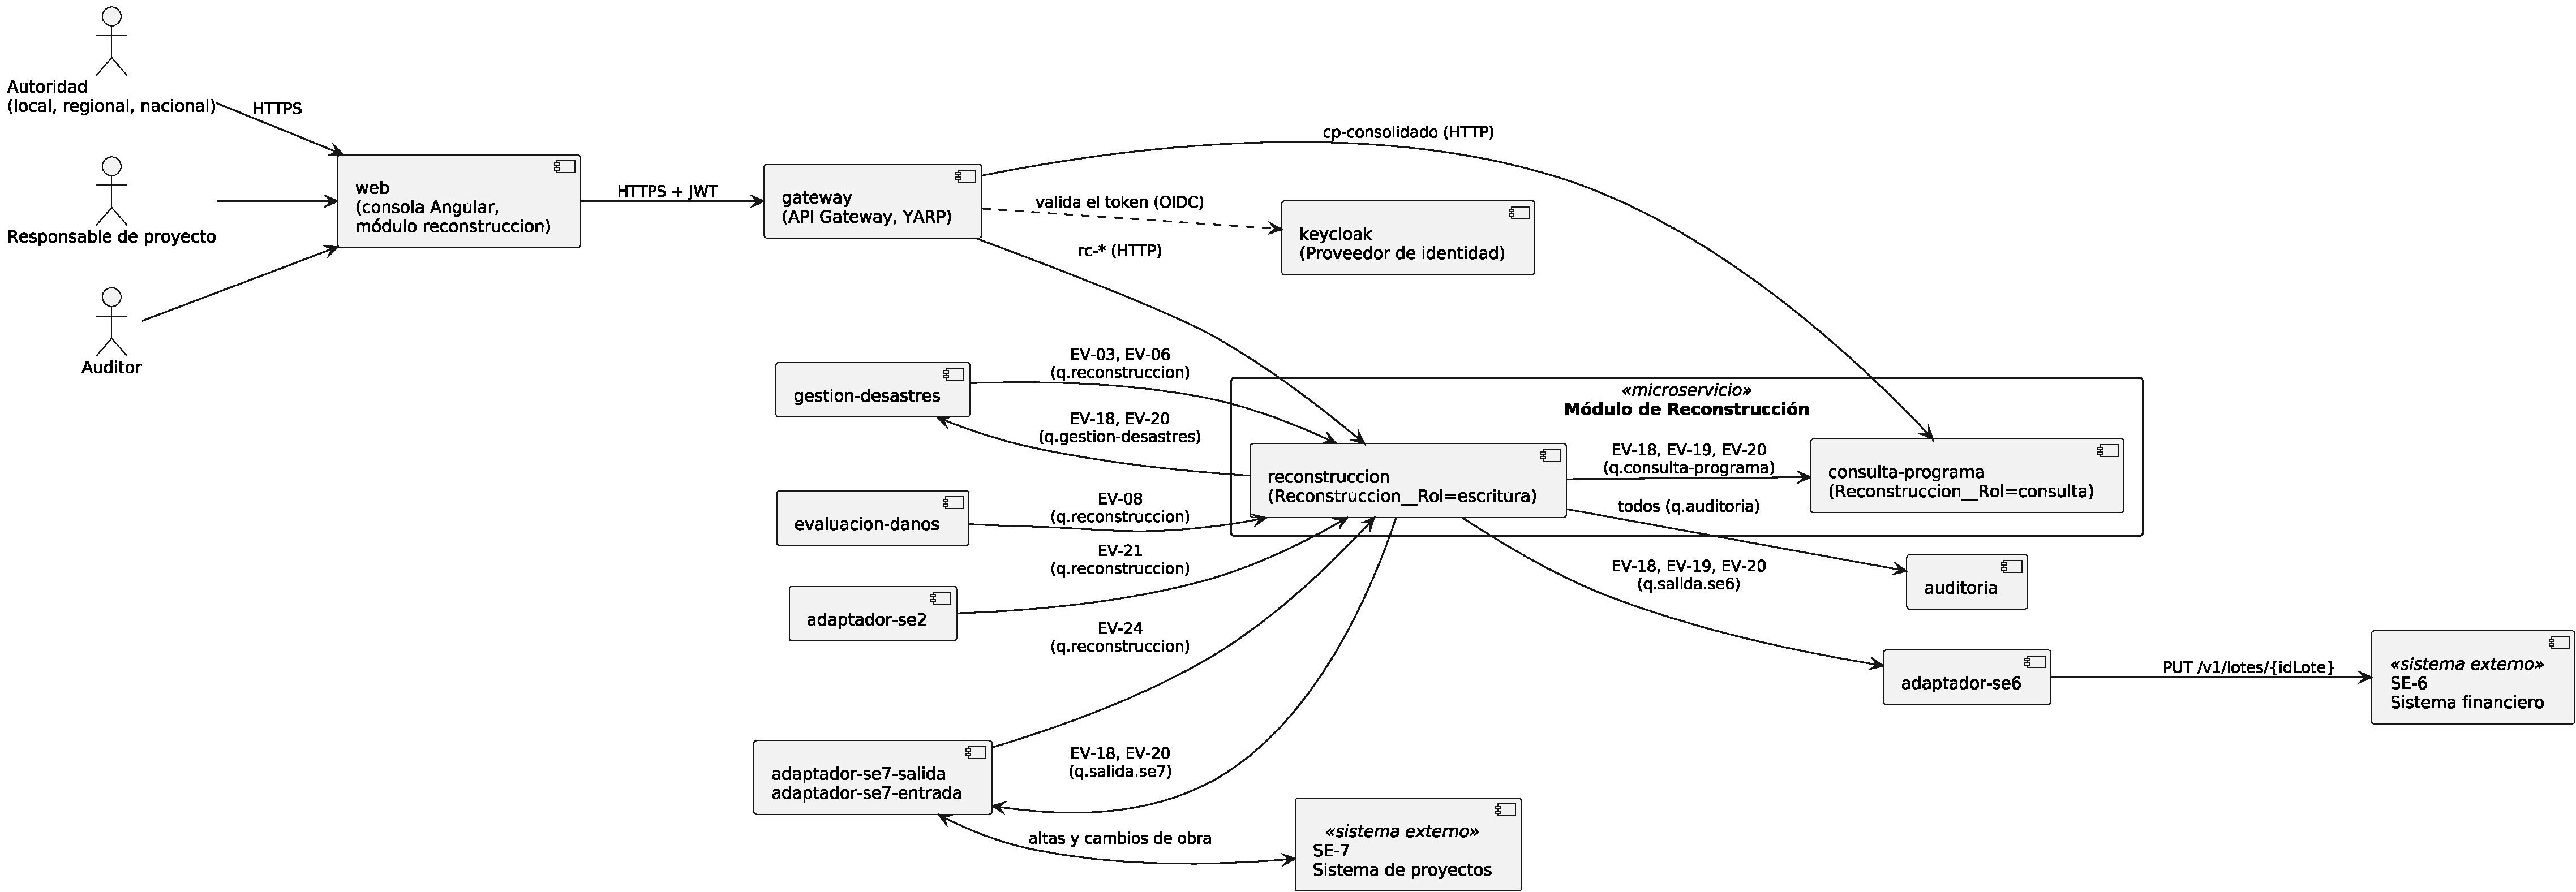
\includegraphics[width=\textwidth]{01-contexto}
  \caption{Contexto del módulo de Reconstrucción}
  \label{fig:contexto}
\end{figure}

\begin{itemize}
  \item \textbf{Autoridad} (local, regional o nacional): consulta candidatas, crea, asigna, aprueba y cancela
        proyectos de su jurisdicción (E-39).
  \item \textbf{Responsable del proyecto}: inicia la ejecución, registra avance, costos y documentos, y finaliza
        el proyecto que tiene asignado.
  \item \textbf{Auditor}: consulta el historial y el consolidado, solo lectura y sin restricción territorial.
  \item Los usuarios entran por la consola \texttt{web} y el \texttt{gateway}. El \texttt{gateway} valida el token
        emitido por \texttt{keycloak} (AD-49, AD-57, AD-58).
  \item \texttt{gestion-desastres} publica EV-03 y EV-06. \texttt{evaluacion-danos} publica EV-08.
        \texttt{adaptador-se2} publica EV-21. El módulo no consulta a ningún otro servicio: guarda copias locales
        de esos datos (AD-46, E-01, E-28, E-36).
  \item El módulo publica EV-18, EV-19 y EV-20 (E-10). Los consumen \texttt{consulta-programa}, \texttt{auditoria},
        \texttt{gestion-desastres} (regla de cierre, AD-47, E-07) y los adaptadores de SE-6 y SE-7.
  \item \texttt{adaptador-se6} entrega presupuesto y costos al sistema financiero SE-6. \texttt{adaptador-se7-salida}
        entrega los proyectos al sistema de proyectos SE-7 y \texttt{adaptador-se7-entrada} publica en EV-24 el
        avance y el contratista que reporta SE-7 (E-04).
\end{itemize}

% ---------------------------------------------------------------------------
\section{Reglas de negocio}
\label{sec:reglas}

{\small
\begin{longtable}{|P{1.7cm}|P{10.6cm}|P{2.3cm}|}
  \hline
  \rowcolor{cabecera}\textbf{ID} & \textbf{Regla} & \textbf{Fuente} \\ \hline
  \endfirsthead
  \hline
  \rowcolor{cabecera}\textbf{ID} & \textbf{Regla} & \textbf{Fuente} \\ \hline
  \endhead
  RN-RC-01 & Un proyecto se crea a partir de una o más evaluaciones de daño \emph{validadas} del mismo desastre. El
    vínculo con cada evaluación de origen nunca se elimina. & RF-RC-01 \\ \hline
  RN-RC-02 & Son candidatas las evaluaciones validadas con daño \emph{grave} o \emph{destrucción total} que no están
    vinculadas a un proyecto vigente. Se leen de la copia local del módulo. & RF-RC-01, E-28 \\ \hline
  RN-RC-03 & Solo se crean proyectos para un desastre en el estado \texttt{EN\_RECONSTRUCCION}. & AD-40 \\ \hline
  RN-RC-04 & Una evaluación está vinculada como máximo a un proyecto que no esté cancelado. & RF-RC-01 \\ \hline
  RN-RC-05 & La creación por lote produce un proyecto por activo evaluado. Si una evaluación incumple una regla, no se
    crea ningún proyecto y se informa cuáles fallaron. Reenviar el lote con la misma \texttt{claveIdempotencia}
    devuelve los mismos proyectos. & RF-RC-08, AD-40 \\ \hline
  RN-RC-06 & El alcance del proyecto se deduce de los municipios (código DIVIPOLA) de sus evaluaciones: uno solo es
    municipal; varios del mismo departamento, regional; varios departamentos, nacional. & DA-14, E-20 \\ \hline
  RN-RC-07 & Un proyecto se crea sin presupuesto ni responsable. Se aprueba solo con presupuesto mayor que cero,
    fuente de financiación, responsable y cronograma con fin posterior al inicio. & RF-RC-03 \\ \hline
  RN-RC-08 & Lo aprueba la autoridad local del municipio si el proyecto es municipal, la autoridad regional del
    departamento si es regional y la autoridad nacional si es nacional. & E-20, DA-14 \\ \hline
  RN-RC-09 & La autoridad solo ve y usa la información de su jurisdicción: la local, la de su municipio; la regional,
    la de los municipios de su departamento; la nacional, todo el territorio. Un proyecto ajeno responde 404 en el
    detalle, el historial y las acciones de la autoridad. Quien ve el proyecto pero no lo aprueba según RN-RC-08
    recibe 403. Un lote con alguna evaluación ajena se rechaza entero con 403. El auditor no tiene restricción
    territorial. & E-39, DA-14 \\ \hline
  RN-RC-10 & Presupuesto, fuente, cronograma y responsable se asignan en \emph{Formulado} y se modifican en
    \emph{Aprobado} o \emph{En ejecución}, siempre con justificación y sin perder las condiciones de RN-RC-07. &
    RF-RC-03 \\ \hline
  RN-RC-11 & Un monto (\texttt{Dinero}) nunca es negativo y admite cero. Un costo registrado es mayor que cero. &
    RF-RC-05 \\ \hline
  RN-RC-12 & Un proyecto aprobado pasa a \emph{En ejecución} cuando tiene contratista, registrado por el responsable o
    recibido de SE-7 (EV-24). & RF-RC-02, E-04 \\ \hline
  RN-RC-13 & El avance y los costos se registran solo \emph{En ejecución}, con autor y fecha. El avance va de 0 a
    100\,\%. Un valor menor que el vigente solo se acepta como corrección justificada. El avance de SE-7 guarda su
    procedencia. & RF-RC-04, E-04 \\ \hline
  RN-RC-14 & Si el costo ejecutado supera el presupuesto, el proyecto queda \emph{en sobrecosto}. La marca no bloquea
    ningún registro. & RF-RC-05 \\ \hline
  RN-RC-15 & Un proyecto se finaliza cuando su avance es 100\,\%. Lo finaliza el responsable asignado. & RF-RC-04 \\
    \hline
  RN-RC-16 & La autoridad cancela un proyecto en cualquier estado no final, con justificación. Sus evaluaciones
    quedan libres y el vínculo se conserva como no vigente. & RF-RC-01 \\ \hline
  RN-RC-17 & \emph{Finalizado} y \emph{Cancelado} son estados finales: no admiten cambios ni documentos. & RF-RC-02 \\
    \hline
  RN-RC-18 & Cada cambio deja una entrada de historial con valor anterior, valor nuevo, autor, justificación, fecha y
    procedencia. Las entradas no se modifican ni se borran. El estado en una fecha pasada se obtiene del
    historial. & RF-RC-07, AD-41 \\ \hline
  RN-RC-19 & La autoridad crea, asigna, aprueba y cancela. Solo el responsable asignado inicia, registra avance,
    costos y documentos, y finaliza su proyecto. El auditor solo consulta. & RF-RC-03 a RF-RC-06 \\ \hline
  RN-RC-20 & Cada cambio se publica como EV-18, EV-19 o EV-20 desde la bandeja de salida de la misma transacción. Si
    SE-6 o SE-7 no responden, la operación se confirma igual y la entrega queda en su cola de salida. &
    AD-45, AD-36 \\ \hline
  RN-RC-21 & El desastre solo se cierra cuando todos sus proyectos están en un estado final. La regla la aplica
    Gestión de Desastres con los eventos EV-18 y EV-20. & AD-47, E-07 \\ \hline
  RN-RC-22 & El consolidado de un desastre muestra proyectos por estado, presupuesto asignado, costo ejecutado y
    avance agregado: promedio de avances ponderado por presupuesto, sin cancelados. & RF-RC-09 \\ \hline
\end{longtable}
}

% ---------------------------------------------------------------------------
\section{Casos de uso}
\label{sec:cu}

\begin{figure}[H]
  \centering
  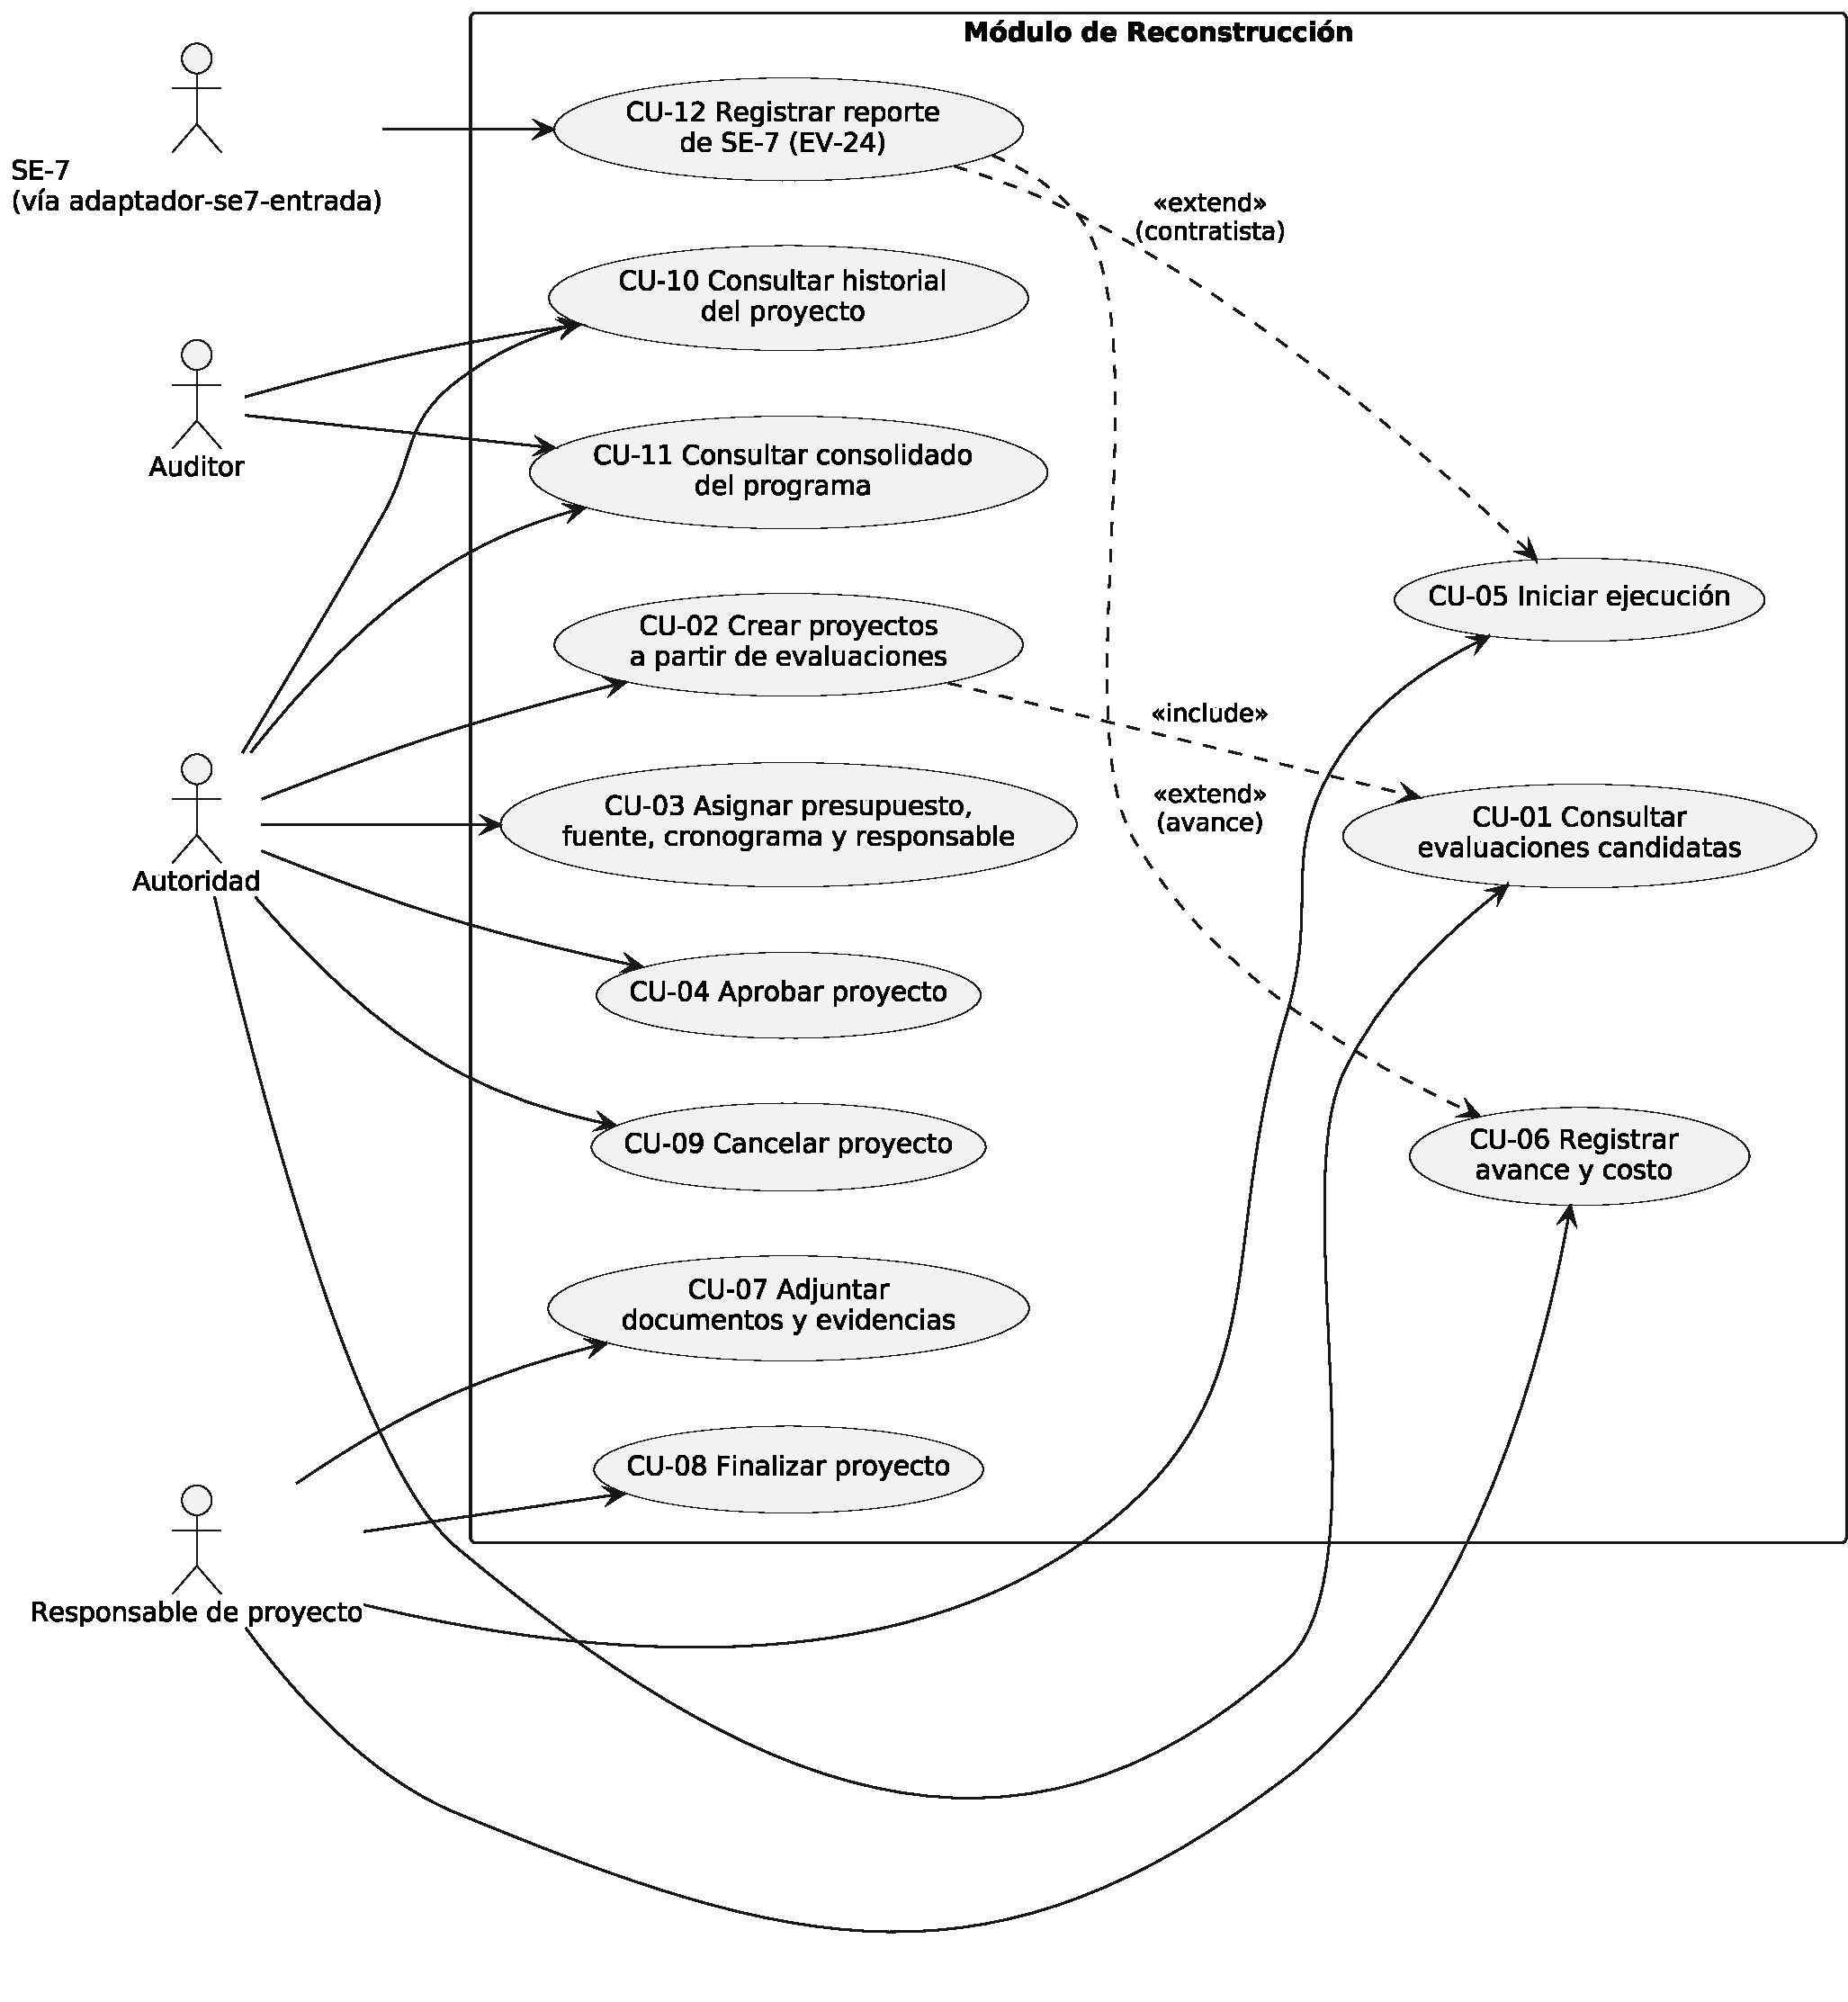
\includegraphics[width=0.95\textwidth]{02-casos-uso}
  \caption{Casos de uso del módulo de Reconstrucción}
  \label{fig:cu}
\end{figure}

Todas las rutas pasan por el \texttt{gateway} con un token JWT (AD-49). Las rutas de proyectos van al servicio
\texttt{reconstruccion} y el consolidado a \texttt{consulta-programa} (catálogo \texttt{rutas.json}, rutas
\texttt{rc-*} y \texttt{cp-consolidado}, E-09). Los casos que cambian un proyecto guardan el proyecto, su entrada
de historial y su evento en una sola transacción (RN-RC-18, RN-RC-20). Las respuestas de error son 403 (rol o
aprobador), 404 (no existe o fuera de jurisdicción, E-39), 409 (transición no permitida, estado final o conflicto
de versión) y 422 (dato que incumple una regla). La última columna indica la precondición de cada caso y sus
excepciones con esos códigos.

{\small
\begin{longtable}{|P{1.8cm}|P{1.9cm}|P{3.1cm}|P{1.2cm}|P{3.3cm}|P{2.9cm}|}
  \hline
  \rowcolor{cabecera}\textbf{Caso de uso} & \textbf{Actor} & \textbf{Ruta} & \textbf{Evento} &
  \textbf{Flujo principal} & \textbf{Precondición y excepciones} \\ \hline
  \endfirsthead
  \hline
  \rowcolor{cabecera}\textbf{Caso de uso} & \textbf{Actor} & \textbf{Ruta} & \textbf{Evento} &
  \textbf{Flujo principal} & \textbf{Precondición y excepciones} \\ \hline
  \endhead
  CU-01 Consultar evaluaciones candidatas & Autoridad
    & {\footnotesize\texttt{GET /v1/reconstruccion/ desastres}}; {\footnotesize\texttt{GET /v1/reconstruccion/ candidatas?desastre=}}
    & Ninguno
    & Elige un desastre en reconstrucción. El sistema lee la copia local alimentada por EV-03, EV-06, EV-08 y
      EV-21 (AD-46) y lista las candidatas de su jurisdicción con activo, tipo, nivel de daño y municipio
      (RN-RC-02, RN-RC-09).
    & Rol autoridad y desastre en reconstrucción. 403 sin el rol. \\ \hline
  CU-02 Crear proyectos a partir de evaluaciones & Autoridad
    & {\footnotesize\texttt{POST /v1/proyectos:lote}} (201)
    & EV-18
    & Envía el desastre, las evaluaciones y la \texttt{claveIdempotencia}. El sistema valida jurisdicción y lote,
      crea un proyecto por activo en \emph{Formulado} y deja un EV-18 por proyecto en la bandeja (AD-45). El relevo
      lo publica y \texttt{adaptador-se7-salida} da de alta la obra en SE-7 (AD-36, AD-37, AD-25). Un reenvío
      devuelve los mismos proyectos (RN-RC-05). Ver figura~\ref{fig:seq-lote}.
    & Evaluaciones validadas y desastre en reconstrucción (RN-RC-03). 403 sin el rol o con una evaluación fuera de la jurisdicción. 422 si una evaluación incumple una regla: no se crea ningún proyecto. \\ \hline
  CU-03 Asignar presupuesto, fuente, cronograma y responsable & Autoridad
    & {\footnotesize\texttt{PATCH /v1/proyectos/\{id\}/ presupuesto}}; {\footnotesize\texttt{PATCH /v1/proyectos/\{id\}/ responsable}}
    & EV-19, EV-20
    & Indica los valores nuevos (presupuesto, fuente y cronograma, o responsable) y la justificación. El sistema
      verifica jurisdicción y estado, guarda valor anterior y nuevo, y deja el evento en la bandeja. EV-19 lleva
      presupuesto y fuente; EV-20 lleva el cronograma y el responsable (E-10). \texttt{adaptador-se6} entrega el
      presupuesto a SE-6 por lotes (AD-36, AD-37).
    & Proyecto en Formulado, Aprobado o En ejecución. 403 sin el rol. 404 fuera de la jurisdicción. 409 en estado final o por conflicto de versión. 422 si falta la justificación o un dato es inválido. \\ \hline
  CU-04 Aprobar proyecto & Autoridad
    & {\footnotesize\texttt{POST /v1/proyectos/\{id\}/ transiciones}} (\texttt{APROBAR})
    & EV-20
    & El sistema verifica que lo ve (si no, 404), datos completos (RN-RC-07) y aprobador (RN-RC-08, si no, 403), y
      pasa el proyecto a \emph{Aprobado}.
    & Proyecto en Formulado, con presupuesto, fuente, responsable y cronograma. 404 si no lo ve. 403 si lo ve y no es quien lo aprueba. 409 en otro estado. 422 si faltan datos. \\ \hline
  CU-05 Iniciar ejecución & Responsable
    & {\footnotesize\texttt{POST /v1/proyectos/\{id\}/ transiciones}} (\texttt{INICIAR})
    & EV-20
    & Registra el contratista o usa el recibido de SE-7 (CU-12) y el proyecto pasa a \emph{En ejecución}
      (RN-RC-12).
    & Proyecto en Aprobado y usuario responsable asignado. 403 si no es el responsable. 409 en otro estado. 422 sin contratista. \\ \hline
  CU-06 Registrar avance y costo & Responsable
    & {\footnotesize\texttt{POST /v1/proyectos/\{id\}/ avance}}
    & EV-20
    & Registra un avance, un costo con su concepto, o ambos. El sistema valida rango y estado, actualiza los
      acumulados y marca sobrecosto si aplica (RN-RC-13, RN-RC-14). EV-20 lleva el avance y el costo, y
      \texttt{adaptador-se6} entrega el costo a SE-6 (E-10). Ver figura~\ref{fig:seq-avance}.
    & Proyecto en En ejecución y usuario responsable asignado. 403 si no es el responsable. 409 en otro estado. 422 con avance fuera de 0 a 100\,\%, costo no positivo o costo sin concepto. \\ \hline
  CU-07 Adjuntar documentos y evidencias & Responsable
    & {\footnotesize\texttt{POST /v1/proyectos/\{id\}/ documentos}} (multipart, $\le$ 25\,MB, 201)
    & EV-20
    & Sube el archivo. El sistema lo guarda en el bucket \texttt{reconstruccion-}\allowbreak\texttt{documentos} con su huella (hash),
      autor y fecha (AD-56).
    & Proyecto que no está en estado final y usuario responsable asignado. 403 si no es el responsable. 409 en estado final. \\ \hline
  CU-08 Finalizar proyecto & Responsable
    & {\footnotesize\texttt{POST /v1/proyectos/\{id\}/ transiciones}} (\texttt{FINALIZAR})
    & EV-20
    & El sistema verifica avance de 100\,\% y pasa el proyecto a \emph{Finalizado} (RN-RC-15).
    & Proyecto en En ejecución. 403 si no es el responsable. 409 en otro estado. 422 si el avance no es 100\,\%. \\ \hline
  CU-09 Cancelar proyecto & Autoridad
    & {\footnotesize\texttt{POST /v1/proyectos/\{id\}/ transiciones}} (\texttt{CANCELAR})
    & EV-20
    & Solicita cancelar con justificación. El proyecto pasa a \emph{Cancelado} y sus evaluaciones quedan libres
      (RN-RC-16).
    & Proyecto que no está en estado final. 404 fuera de la jurisdicción. 409 en estado final. 422 sin justificación. \\ \hline
  CU-10 Consultar historial del proyecto & Auditor, autoridad
    & {\footnotesize\texttt{GET /v1/proyectos/\{id\}/ historial?fecha=}}
    & Ninguno
    & El sistema devuelve las entradas en orden y, si se indica la fecha, el proyecto como estaba en ella
      (RN-RC-18, AD-41).
    & Rol auditor o autoridad. 404 si el proyecto no existe o está fuera de la jurisdicción. \\ \hline
  CU-11 Consultar consolidado del programa & Autoridad, auditor
    & {\footnotesize\texttt{GET /v1/programa/ consolidado?desastre=}}
    & Consume EV-18, EV-19, EV-20
    & \texttt{consulta-programa} responde desde su proyección: proyectos por estado, presupuesto, costo, avance
      agregado, proyectos en sobrecosto y la marca de tiempo del dato (RN-RC-22, AD-42).
    & Rol autoridad o auditor. 403 sin el rol. La autoridad solo ve su jurisdicción. \\ \hline
  CU-12 Registrar reporte de SE-7 & SE-7 (vía adaptador)
    & Ninguna (cola \texttt{q.reconstruccion})
    & Consume EV-24; produce EV-20
    & El adaptador consulta los cambios de SE-7 cada 30\,s y publica EV-24. El módulo registra el contratista o el
      avance con procedencia SE-7 (RN-RC-12, RN-RC-13, E-04) y publica EV-20. Si el proyecto está en un estado que
      no admite el cambio, el reporte se descarta con su motivo.
    & Evento EV-24 recibido. Si el proyecto no admite el cambio, el reporte se descarta con su motivo. \\ \hline
\end{longtable}
}

También se consultan {\footnotesize\texttt{GET /v1/proyectos?desastre=}} (lista) y {\footnotesize\texttt{GET /v1/proyectos/\{id\}}} (detalle),
filtrados por jurisdicción (RN-RC-09).

% ---------------------------------------------------------------------------
\section{Entidades}
\label{sec:entidades}

Las entidades son el centro de la arquitectura limpia. Guardan las reglas de negocio y no conocen casos de uso, base
de datos ni framework (AD-08). Viven en el proyecto \texttt{Reconstruccion.\allowbreak Dominio}, que no depende de ningún paquete
externo. La figura~\ref{fig:clases} usa los nombres del código.

\begin{figure}[H]
  \centering
  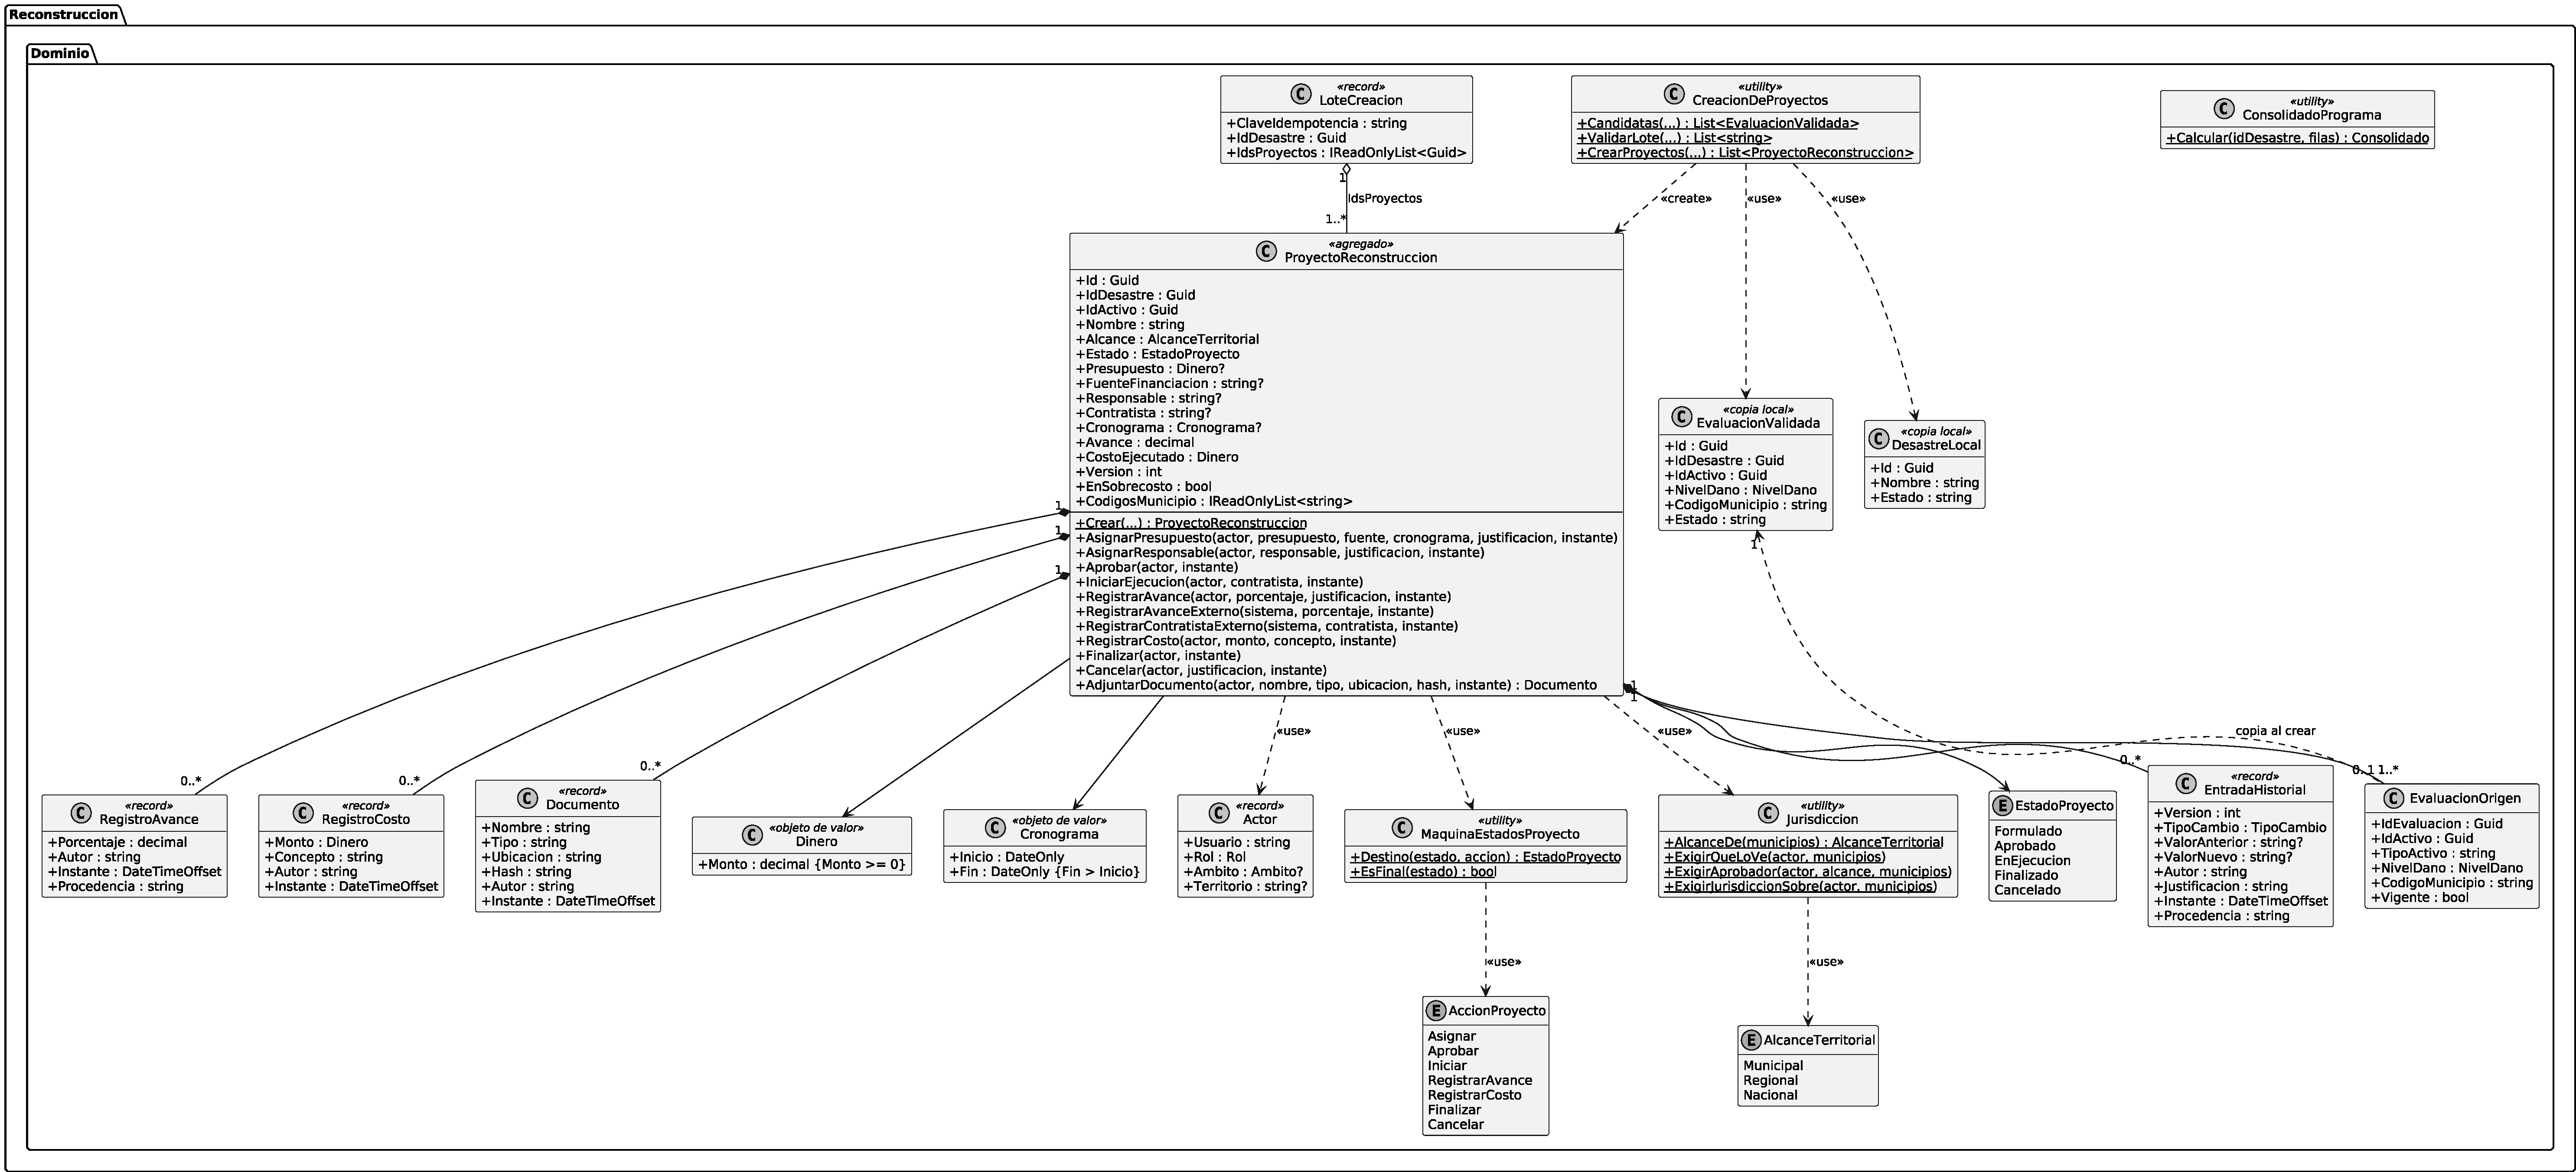
\includegraphics[width=\textwidth]{03-clases-dominio}
  \caption{Diagrama de clases del dominio (\texttt{Reconstruccion.\allowbreak Dominio})}
  \label{fig:clases}
\end{figure}

{\small
\begin{longtable}{|P{3.9cm}|P{6.4cm}|P{4.3cm}|}
  \hline
  \rowcolor{cabecera}\textbf{Clase} & \textbf{Qué representa} & \textbf{Reglas que aplica} \\ \hline
  \endfirsthead
  \hline
  \rowcolor{cabecera}\textbf{Clase} & \textbf{Qué representa} & \textbf{Reglas que aplica} \\ \hline
  \endhead
  \texttt{ProyectoReconstruccion} & Agregado con desastre, activo, alcance, estado, presupuesto, fuente, responsable,
    contratista, cronograma, avance, costo ejecutado y versión. Un método por operación. Acumula sus entradas de
    historial nuevas. & RN-RC-07 a RN-RC-19 \\ \hline
  \texttt{MaquinaEstadosProyecto} & Tabla de transiciones por \texttt{EstadoProyecto} y \texttt{AccionProyecto}
    (sección~\ref{sec:estados}). & Ninguna transición fuera de la tabla \\ \hline
  \texttt{Jurisdiccion} & Alcance por municipios DIVIPOLA y reglas de visibilidad y aprobación. & RN-RC-06,
    RN-RC-08, RN-RC-09 \\ \hline
  \texttt{CreacionDeProyectos} & Candidatas, validación del lote y creación de un proyecto por activo. & RN-RC-01 a
    RN-RC-05 \\ \hline
  \texttt{EvaluacionOrigen} & Activo, tipo, nivel de daño y municipio de la evaluación que originó el proyecto, con
    su marca de vigencia. & RN-RC-01, RN-RC-16 \\ \hline
  \texttt{EntradaHistorial} & Cambio con versión, tipo, valor anterior y nuevo, autor, justificación, instante y
    procedencia. & RN-RC-18 \\ \hline
  \texttt{RegistroAvance}, \texttt{RegistroCosto}, \texttt{Documento} & Avances, costos y archivos con autor y
    fecha. & RN-RC-13, RN-RC-14, RN-RC-17 \\ \hline
  \texttt{LoteCreacion} & Lote con su \texttt{ClaveIdempotencia} y los proyectos que creó. & RN-RC-05 \\ \hline
  \texttt{Dinero}, \texttt{Cronograma} & Objetos de valor: monto en pesos mayor o igual que cero; fechas con fin
    posterior al inicio. & RN-RC-07, RN-RC-11 \\ \hline
  \texttt{Actor} & Usuario, rol, ámbito y territorio que la capa de acceso arma con el token. & RN-RC-09, RN-RC-19
    \\ \hline
  \texttt{DesastreLocal}, \texttt{EvaluacionValidada} & Copias locales de datos de otros módulos, alimentadas por
    eventos (AD-46). & RN-RC-02, RN-RC-03 \\ \hline
  \texttt{ConsolidadoPrograma}, \texttt{ReconstruccionHistorica} & Cálculo del consolidado y estado en una fecha
    a partir del historial. & RN-RC-22, RN-RC-18 \\ \hline
\end{longtable}
}

% ---------------------------------------------------------------------------
\section{Diagrama de transición de estados}
\label{sec:estados}

\begin{figure}[H]
  \centering
  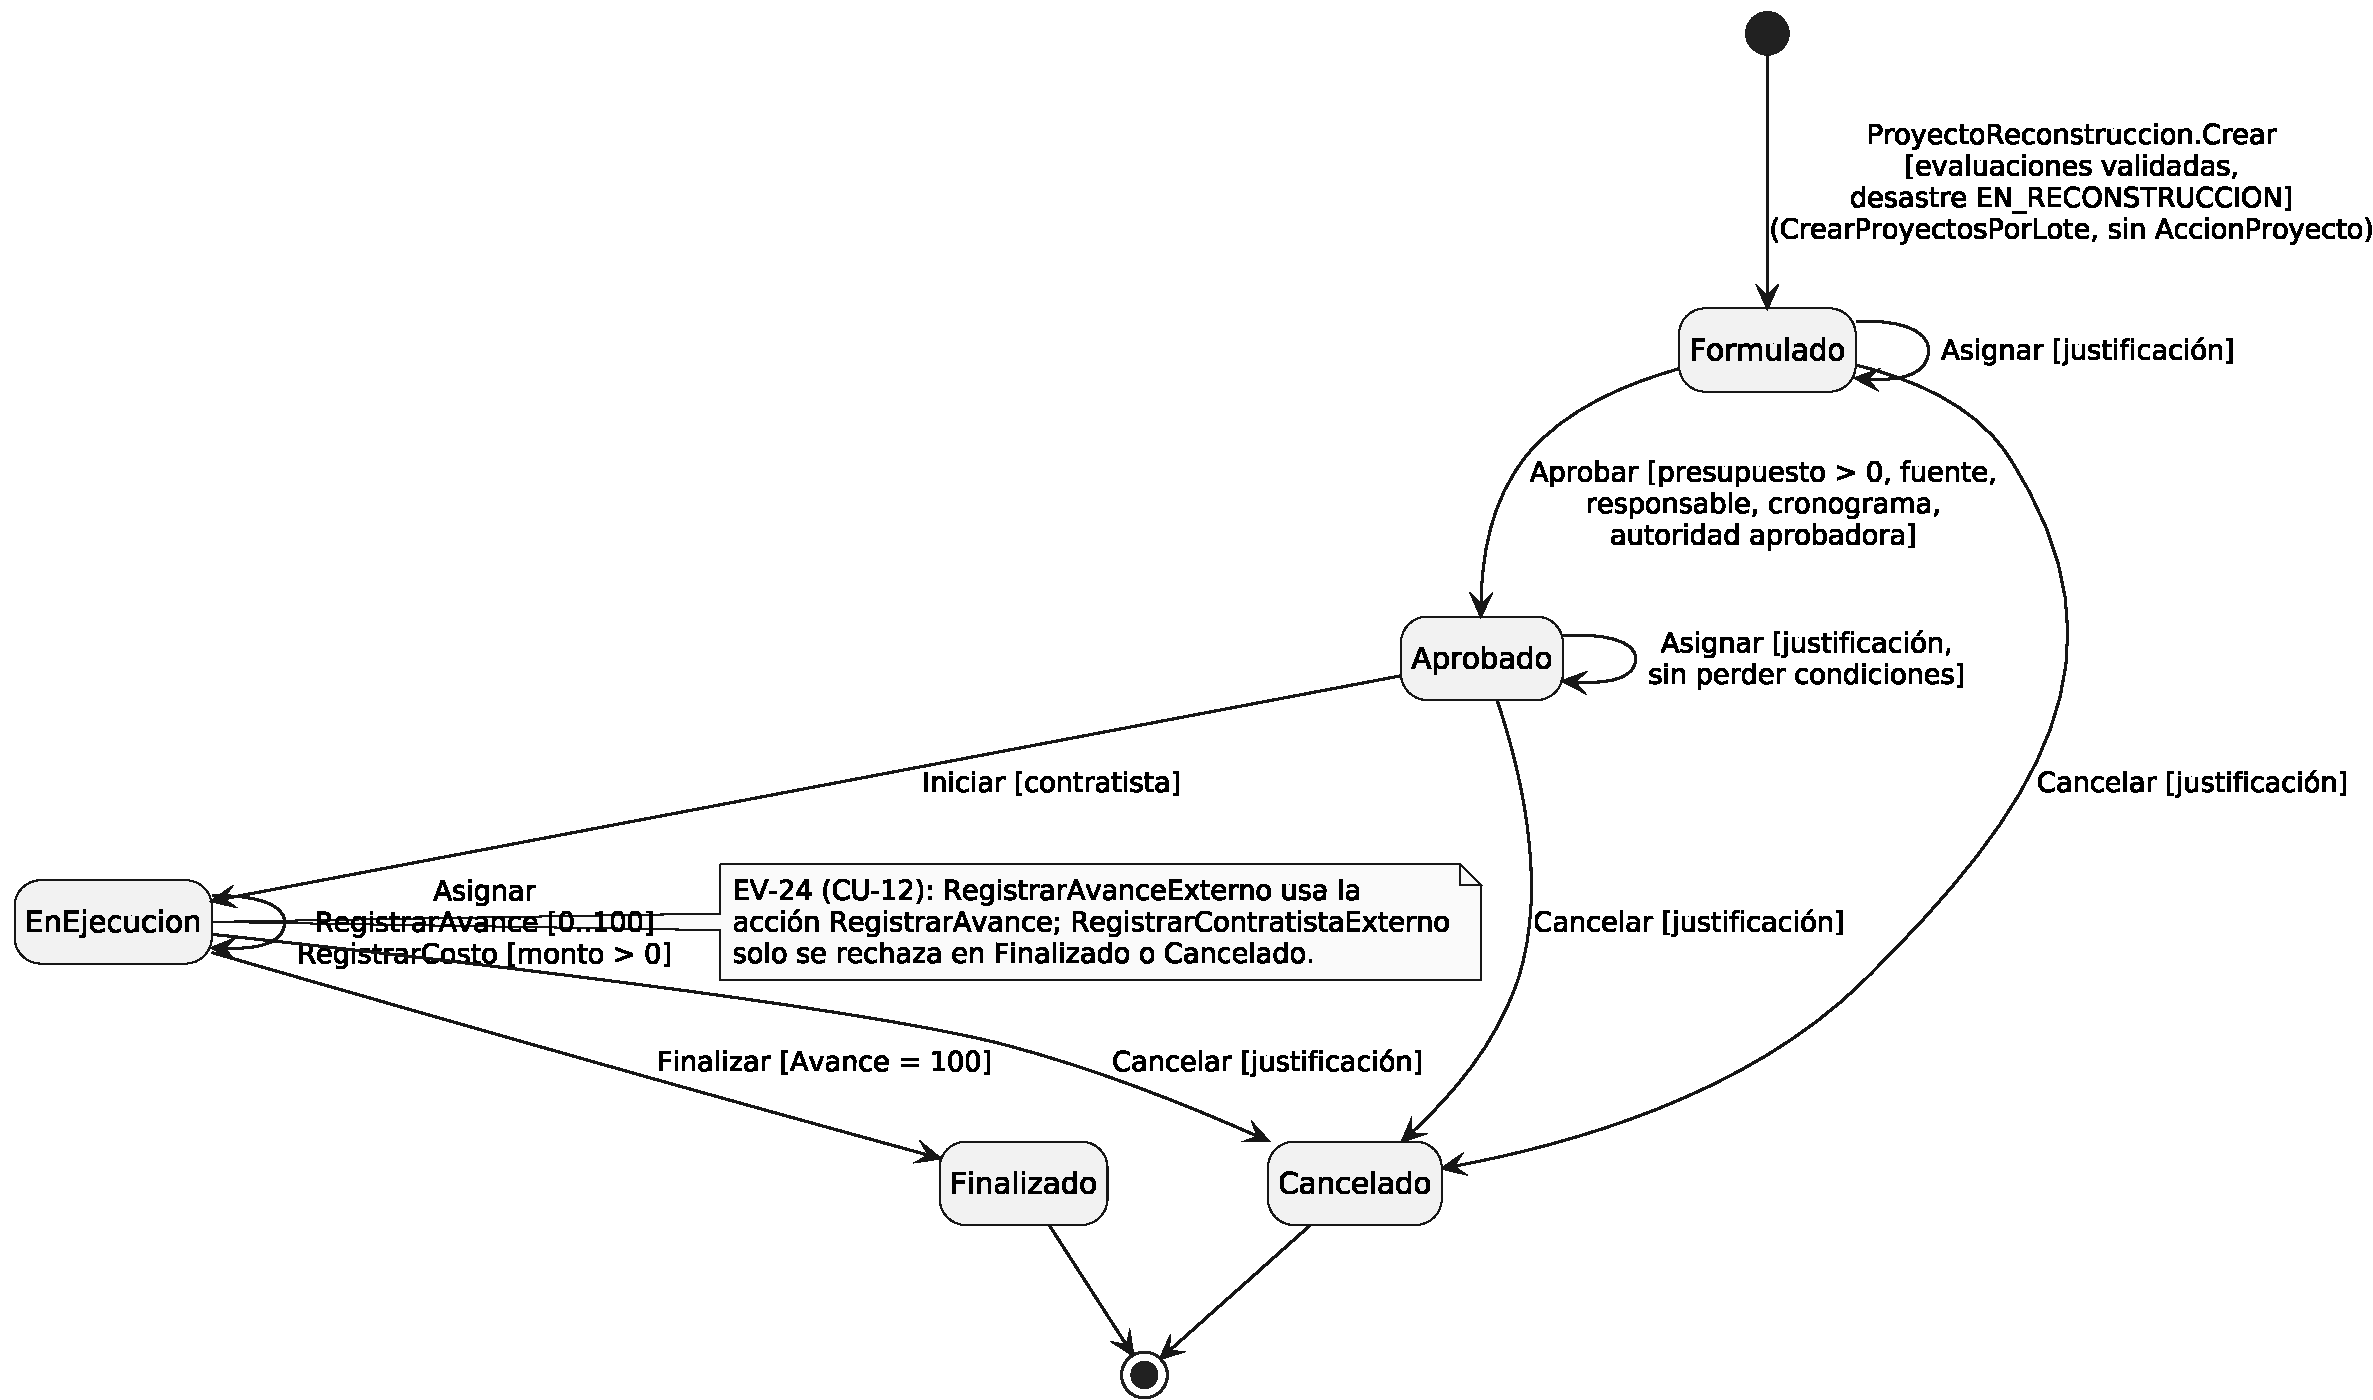
\includegraphics[width=0.9\textwidth]{04-estados-proyecto}
  \caption{Máquina de estados de \texttt{ProyectoReconstruccion}}
  \label{fig:estados}
\end{figure}

La creación no es una \texttt{AccionProyecto}. La hace \texttt{ProyectoReconstruccion.Crear}, invocado por
\texttt{CreacionDeProyectos.CrearProyectos} dentro de CU-02, y deja la entrada de historial de tipo
\texttt{Creacion}. Las demás transiciones están en \texttt{MaquinaEstadosProyecto}:

{\small
\begin{longtable}{|P{2.7cm}|P{3.2cm}|P{2.3cm}|P{3.9cm}|P{2.0cm}|}
  \hline
  \rowcolor{cabecera}\textbf{AccionProyecto} & \textbf{Desde} & \textbf{Hacia} & \textbf{Condición} &
  \textbf{Quién} \\ \hline
  \endfirsthead
  \hline
  \rowcolor{cabecera}\textbf{AccionProyecto} & \textbf{Desde} & \textbf{Hacia} & \textbf{Condición} &
  \textbf{Quién} \\ \hline
  \endhead
  (creación) & inicio & Formulado & RN-RC-01 a RN-RC-05 & Autoridad \\ \hline
  \texttt{Asignar} & Formulado, Aprobado, EnEjecucion & el mismo & Justificación; RN-RC-10 & Autoridad \\ \hline
  \texttt{Aprobar} & Formulado & Aprobado & RN-RC-07 y RN-RC-08 & Autoridad \\ \hline
  \texttt{Iniciar} & Aprobado & EnEjecucion & Contratista (RN-RC-12) & Responsable \\ \hline
  \texttt{RegistrarAvance} & EnEjecucion & EnEjecucion & Avance de 0 a 100\,\% & Responsable o SE-7 \\ \hline
  \texttt{RegistrarCosto} & EnEjecucion & EnEjecucion & Monto mayor que cero & Responsable \\ \hline
  \texttt{Registrar\allowbreak Contratista\allowbreak Externo} (método, sin acción propia) & Formulado, Aprobado, EnEjecucion & el mismo & Reporte de SE-7
    (EV-24) & SE-7 \\ \hline
  \texttt{Finalizar} & EnEjecucion & Finalizado & Avance de 100\,\% & Responsable \\ \hline
  \texttt{Cancelar} & Formulado, Aprobado, EnEjecucion & Cancelado & Justificación & Autoridad \\ \hline
\end{longtable}
}

El avance que reporta SE-7 (\texttt{RegistrarAvanceExterno}) usa la acción \texttt{RegistrarAvance}. El contratista que
reporta SE-7 (\texttt{RegistrarContratistaExterno}) no es una \texttt{AccionProyecto}: no cambia el estado y solo se
rechaza si el proyecto está en \emph{Finalizado} o \emph{Cancelado}.

Una acción que no está en la tabla para el estado actual lanza \texttt{TRANSICION\_NO\_PERMITIDA} (409) y no deja
historial. Cada transición aceptada guarda su entrada de historial y su evento en la misma transacción (AD-45).
Cuando todos los proyectos de un desastre llegan a \emph{Finalizado} o \emph{Cancelado}, Gestión de Desastres
permite cerrarlo (RN-RC-21, AD-47).

% ---------------------------------------------------------------------------
\section{Arquitectura limpia y vista lógica}
\label{sec:logica}

\subsection{Anillos y capas}

El módulo sigue la arquitectura limpia \cite{martin}. Sus anillos se corresponden con las cuatro capas del microservicio tipo del
SAD (AD-08). Cada anillo es un proyecto .NET y la regla de dependencia se verifica con
\texttt{PruebasArquitectura} (\texttt{Reconstruccion.\allowbreak Pruebas}), que falla si el dominio usa otro proyecto o paquete,
o si la aplicación usa algo distinto del dominio (QA-10).

{\small
\begin{longtable}{|P{3.0cm}|P{2.8cm}|P{3.6cm}|P{5.2cm}|}
  \hline
  \rowcolor{cabecera}\textbf{Anillo} & \textbf{Capa (AD-08)} & \textbf{Proyecto} & \textbf{Elementos} \\ \hline
  \endfirsthead
  \hline
  \rowcolor{cabecera}\textbf{Anillo} & \textbf{Capa (AD-08)} & \textbf{Proyecto} & \textbf{Elementos} \\ \hline
  \endhead
  Entidades & Dominio & \texttt{Reconstruccion.\allowbreak Dominio} & Clases de la figura~\ref{fig:clases}. \\ \hline
  Casos de uso & Acceso & \texttt{Reconstruccion.\allowbreak Aplicacion} & Interactores, \texttt{GuardadoDeProyectos} y
    puertos (\texttt{IPuertoEntrada}, \texttt{IPuertoSalida}, \texttt{IRepositorioProyectos}, etc.). \\ \hline
  Adaptadores de interfaz (entrada) & Acceso & \texttt{Reconstruccion.\allowbreak Api} & \texttt{ProyectosController},
    \texttt{ProgramaController}, \texttt{PresentadorHttp<T>}. \\ \hline
  Adaptadores de interfaz (salida) & Infraestructura & \texttt{Reconstruccion.\allowbreak Infraestructura} & Gateways EF Core,
    \texttt{PublicadorHechosBandeja}, \texttt{AlmacenDocumentosMinio}, manejadores de eventos. \\ \hline
  Frameworks y drivers & Infraestructura y presentación & \texttt{comun}, \texttt{consola} & ASP.NET Core,
    EF Core, \texttt{Plataforma.Comun.Mensajeria}, RabbitMQ, PostgreSQL, MinIO, consola Angular. \\ \hline
\end{longtable}
}

\subsection{Vista lógica}

\begin{figure}[H]
  \centering
  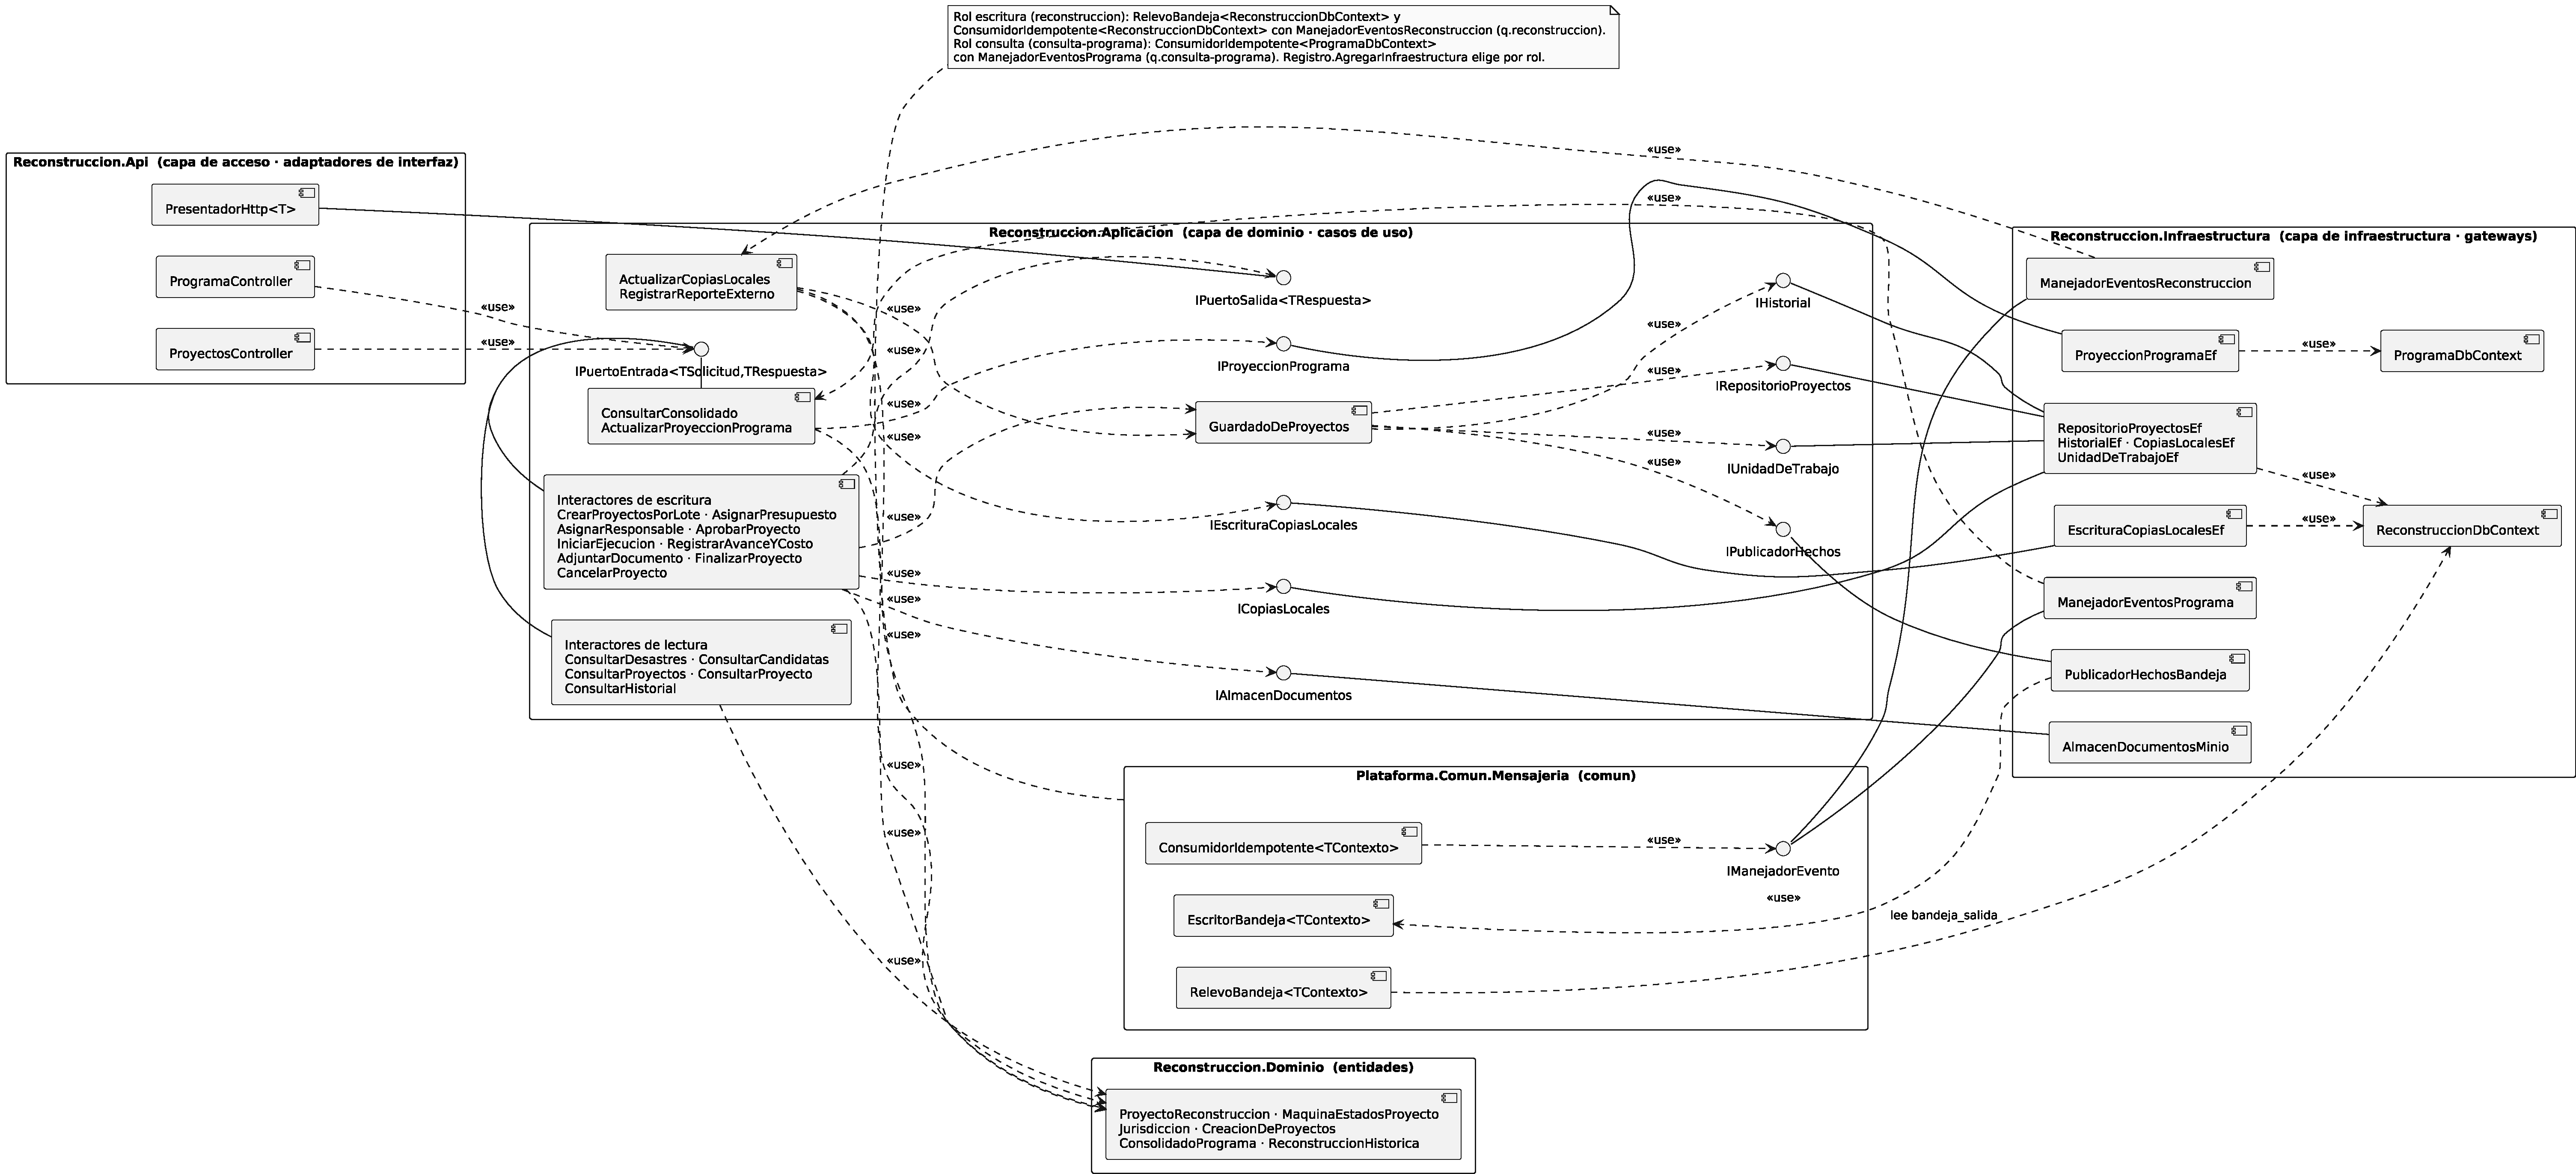
\includegraphics[width=\textwidth]{05-vista-logica}
  \caption{Vista lógica: componentes e interfaces del módulo (UML de componentes)}
  \label{fig:logica}
\end{figure}

La figura~\ref{fig:logica} dibuja los puertos como interfaces UML. El componente que la implementa la ofrece
(línea con círculo) y el que la usa depende de ella (\texttt{<<use>>}). Las dependencias apuntan hacia el dominio.

{\small
\begin{longtable}{|P{4.2cm}|P{6.4cm}|P{4.0cm}|}
  \hline
  \rowcolor{cabecera}\textbf{Elemento} & \textbf{Responsabilidad} & \textbf{Interfaces} \\ \hline
  \endfirsthead
  \hline
  \rowcolor{cabecera}\textbf{Elemento} & \textbf{Responsabilidad} & \textbf{Interfaces} \\ \hline
  \endhead
  \texttt{ProyectosController} & Rutas \texttt{rc-*}. Arma el \texttt{Actor} con el token (nivel 2 de AD-49) y
    llama al puerto de entrada. & Usa \texttt{IPuertoEntrada} \\ \hline
  \texttt{ProgramaController} & Ruta \texttt{cp-consolidado} en el rol consulta. & Usa \texttt{IPuertoEntrada} \\
    \hline
  \texttt{PresentadorHttp<T>} & Convierte el resultado en 200, 201, 403, 404, 409 o 422. & Ofrece
    \texttt{IPuertoSalida} \\ \hline
  Interactores & Un caso de uso cada uno. Coordinan entidades y puertos; no tienen reglas propias. & Ofrecen
    \texttt{IPuertoEntrada} \\ \hline
  \texttt{GuardadoDeProyectos} & Guarda proyecto, historial, eventos y lote en una transacción. & Usa
    \texttt{IRepositorioProyectos}, \texttt{IHistorial}, \texttt{IPublicadorHechos}, \texttt{IUnidadDeTrabajo} \\
    \hline
  \texttt{RepositorioProyectosEf}, \texttt{HistorialEf}, \texttt{CopiasLocalesEf}, \texttt{UnidadDeTrabajoEf} &
    Gateways sobre \texttt{ReconstruccionDbContext}. \texttt{UnidadDeTrabajoEf} convierte un conflicto de versión
    en 409. & Ofrecen los puertos homónimos \\ \hline
  \texttt{PublicadorHechosBandeja} & Traduce cada hecho a EV-18, EV-19 o EV-20 y lo escribe en la bandeja con
    \texttt{EscritorBandeja<TContexto>}. & Ofrece \texttt{IPublicadorHechos} \\ \hline
  \texttt{AlmacenDocumentosMinio} & Guarda los archivos en MinIO. & Ofrece \texttt{IAlmacenDocumentos} \\ \hline
  \texttt{ManejadorEventos\allowbreak Reconstruccion} & Traduce EV-03, EV-06, EV-08, EV-21 y EV-24 de
    \texttt{q.reconstruccion} a \texttt{ActualizarCopiasLocales} y \texttt{RegistrarReporteExterno}. & Ofrece
    \texttt{IManejadorEvento} \\ \hline
  \texttt{ManejadorEventos\allowbreak Programa} & Traduce EV-18, EV-19 y EV-20 de \texttt{q.consulta-programa} a
    \texttt{ActualizarProyeccionPrograma}. EV-23 llega a la misma cola y no se proyecta. & Ofrece
    \texttt{IManejadorEvento} \\ \hline
  \texttt{ProyeccionProgramaEf} & Modelo de lectura en \texttt{ProgramaDbContext}; aplica una fila solo si su versión
    es mayor. & Ofrece \texttt{IProyeccionPrograma} \\ \hline
  \texttt{RelevoBandeja\allowbreak <TContexto>}, \texttt{Consumidor\allowbreak Idempotente\allowbreak <TContexto>} & Servicios en segundo plano de
    \texttt{Plataforma.Comun.Mensajeria}: publican la bandeja y consumen la cola sin repetir mensajes. & Usa
    \texttt{IManejadorEvento} \\ \hline
\end{longtable}
}

La misma imagen \texttt{plataforma/reconstruccion} corre en dos roles (AD-42). Con
\texttt{Reconstruccion\_\_Rol=escritura}, \texttt{Registro.AgregarInfraestructura} registra los gateways, la bandeja,
el relevo y el consumidor de \texttt{q.reconstruccion}. Con \texttt{Reconstruccion\_\_Rol=consulta} registra solo
\texttt{ProyeccionProgramaEf} y el consumidor de \texttt{q.consulta-programa}. La consola es una sola aplicación
Angular (\texttt{consola}) con el módulo \texttt{modulos/reconstruccion} y sus páginas \texttt{candidatas},
\texttt{proyectos}, \texttt{proyecto} y \texttt{consolidado} (AD-59).

% ---------------------------------------------------------------------------
\section{Vista de procesos}
\label{sec:procesos}

{\small
\begin{longtable}{|P{3.4cm}|P{3.6cm}|P{3.6cm}|P{4.0cm}|}
  \hline
  \rowcolor{cabecera}\textbf{Cola} & \textbf{Eventos} & \textbf{Consumidor} & \textbf{Propósito} \\ \hline
  \endfirsthead
  \hline
  \rowcolor{cabecera}\textbf{Cola} & \textbf{Eventos} & \textbf{Consumidor} & \textbf{Propósito} \\ \hline
  \endhead
  \texttt{q.reconstruccion} & EV-03, EV-06, EV-08, EV-21, EV-24 & \texttt{reconstruccion} & Copias locales (AD-46)
    y CU-12 (E-04) \\ \hline
  \texttt{q.consulta-programa} & EV-18, EV-19, EV-20, EV-23 & \texttt{consulta-programa} & Proyección del
    consolidado (AD-42) \\ \hline
  \texttt{q.gestion-desastres} & EV-18, EV-20 (y EV-21) & \texttt{gestion-desastres} & Regla de cierre (AD-47,
    E-07) \\ \hline
  \texttt{q.salida.se6} & EV-18, EV-19, EV-20 & \texttt{adaptador-se6} & Entrega por lotes a SE-6 (AD-36, AD-37,
    E-10) \\ \hline
  \texttt{q.salida.se7} & EV-18, EV-20 & \texttt{adaptador-se7-salida} & Alta y cambio de obra en SE-7 (AD-36,
    AD-37) \\ \hline
  \texttt{q.auditoria} & todos & \texttt{auditoria} & Registro de auditoría (QA-13) \\ \hline
\end{longtable}
}

Todas las colas son quorum y acotadas, ligadas al exchange \texttt{plataforma.eventos} con claves
\texttt{evNN.\#}. Cada una tiene su \texttt{dlq.*} en \texttt{plataforma.dlx} (AD-02, AD-54,
\texttt{despliegue/bus/definiciones.json}).

\begin{figure}[p]
  \centering
  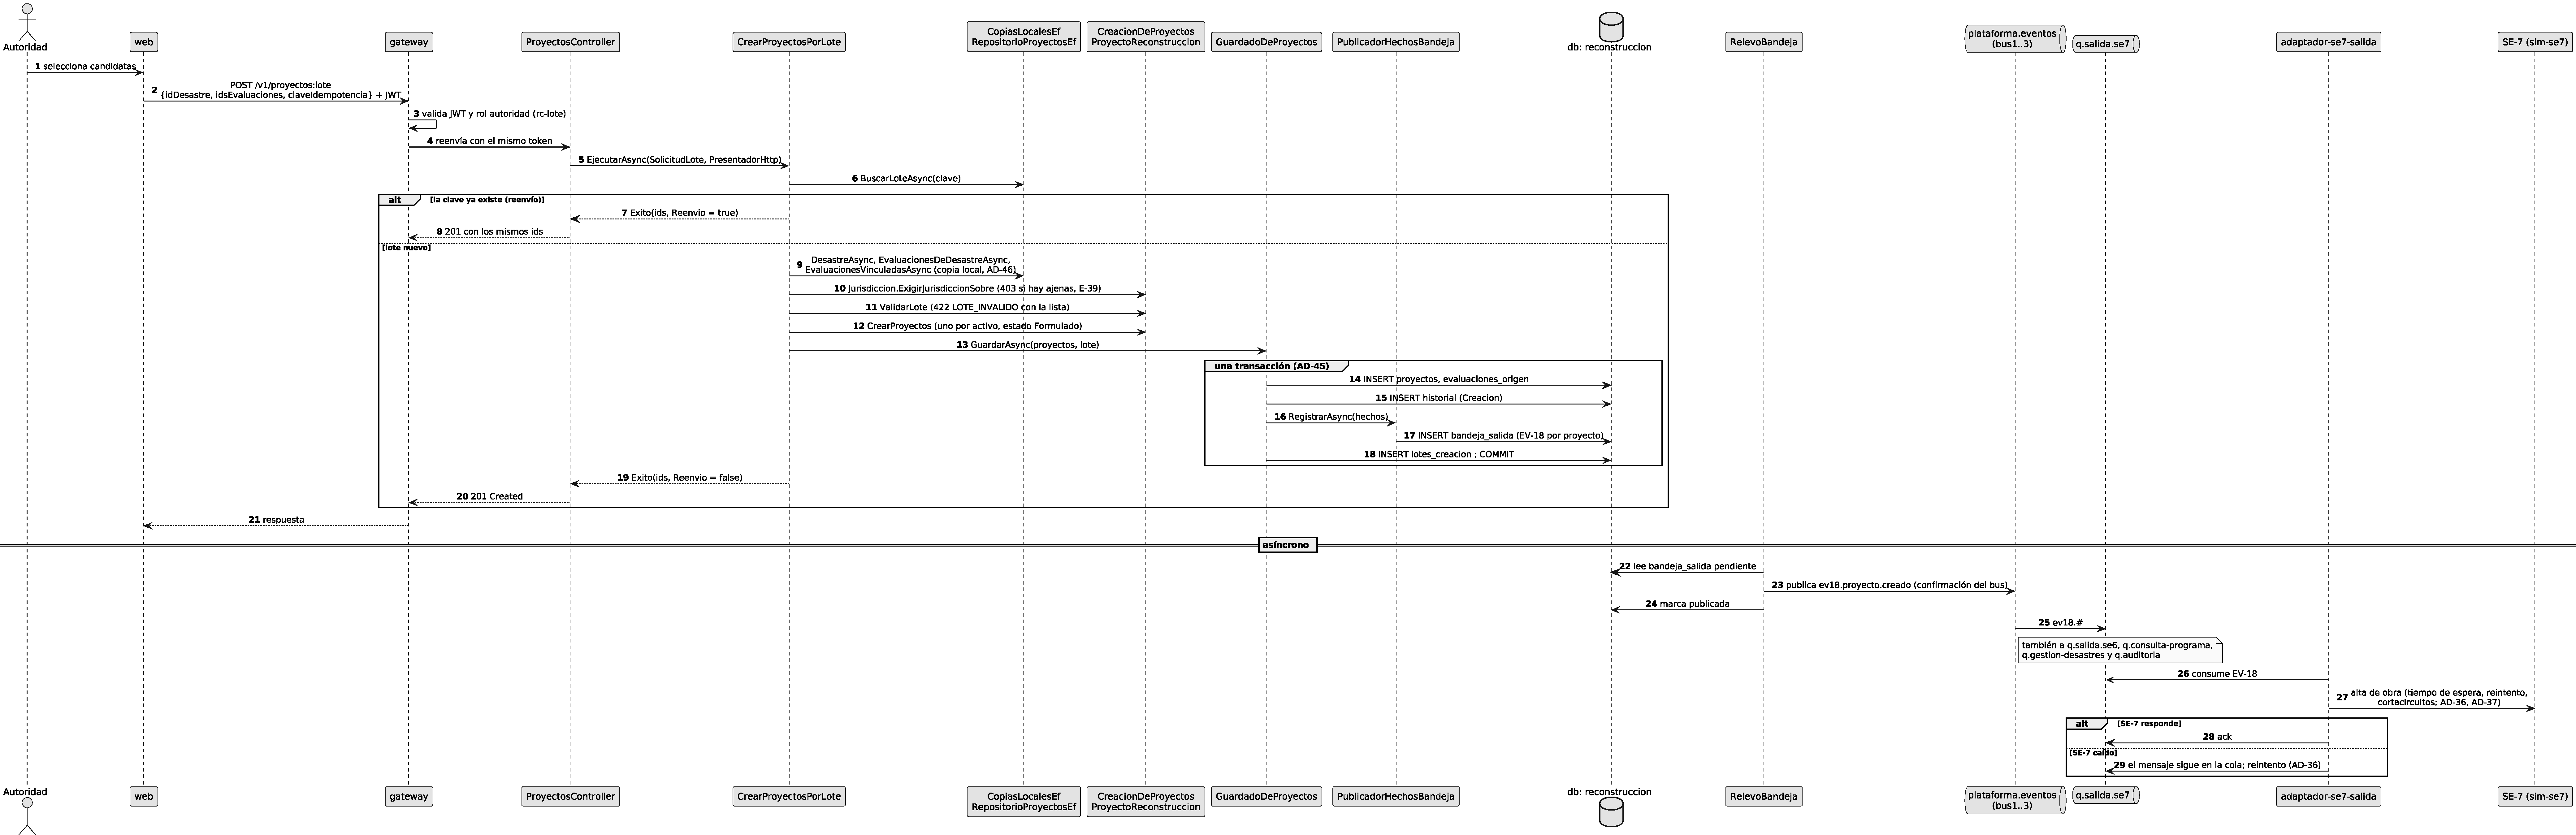
\includegraphics[width=0.86\textheight,height=\textwidth,keepaspectratio,angle=90]{06-secuencia-lote}
  \caption{Secuencia de CU-02: lote, transacción con bandeja, relevo, \texttt{q.salida.se7} y SE-7}
  \label{fig:seq-lote}
\end{figure}

\begin{figure}[p]
  \centering
  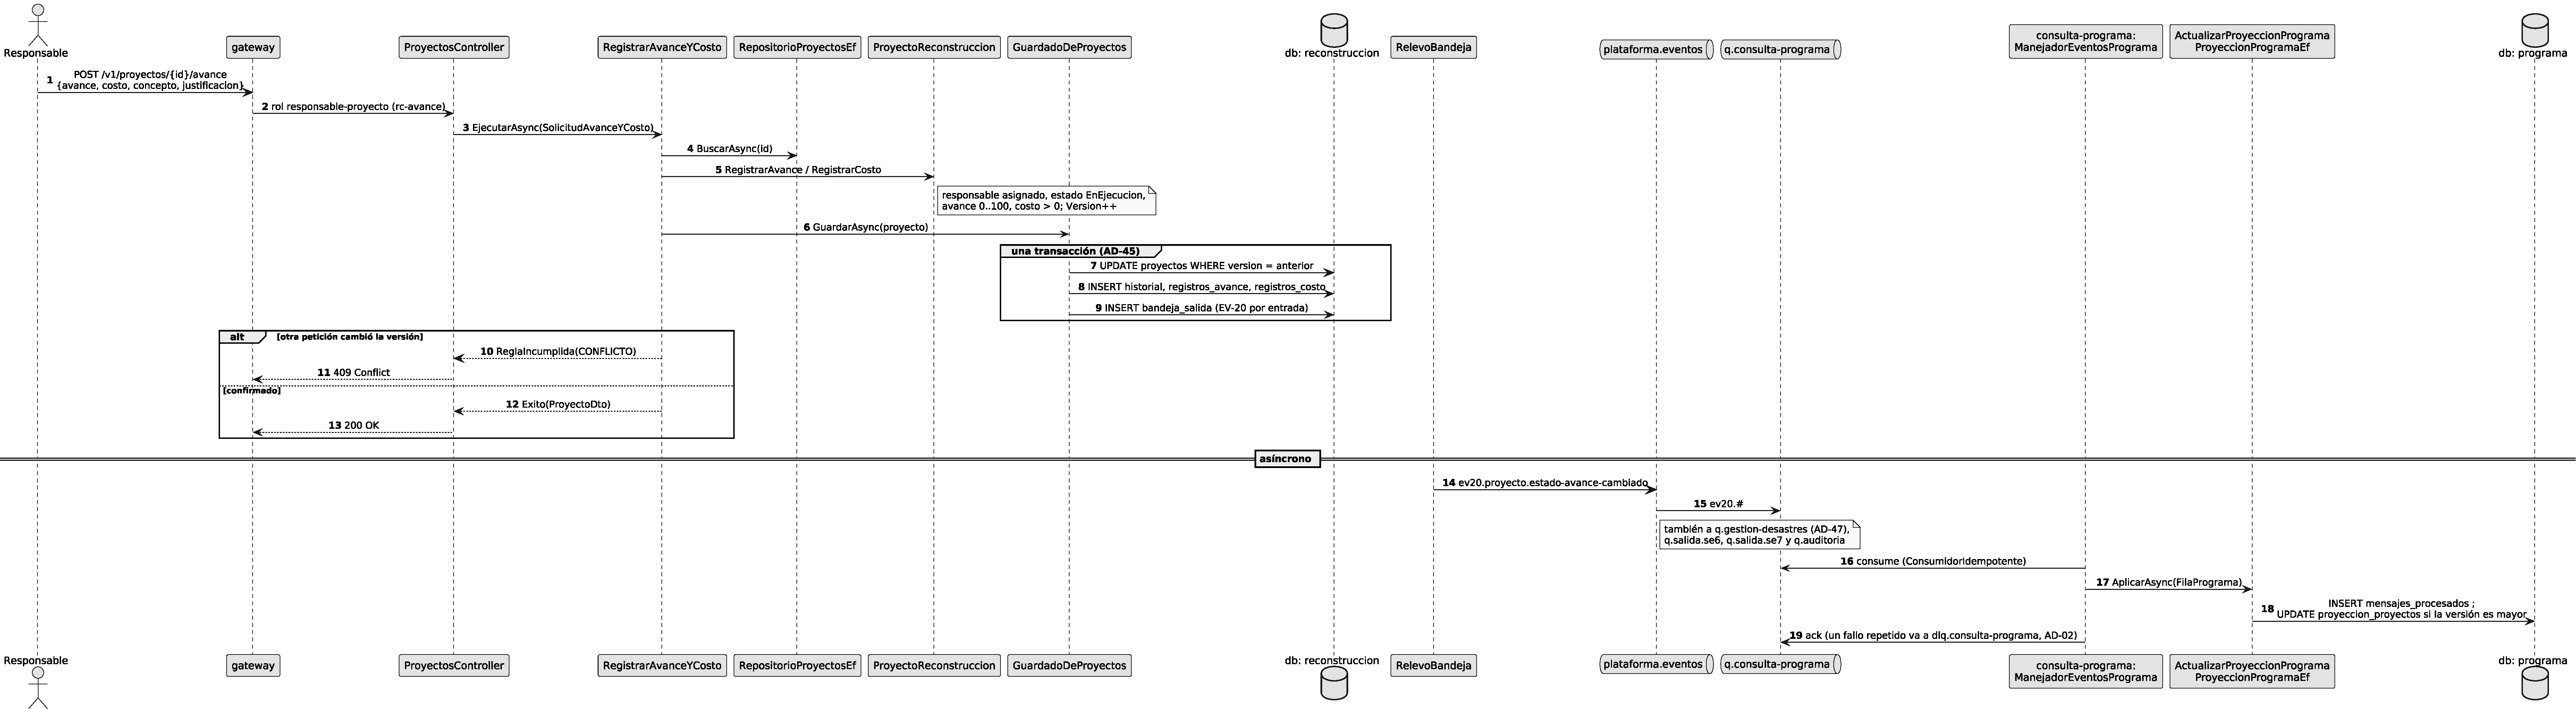
\includegraphics[width=0.86\textheight,height=\textwidth,keepaspectratio,angle=90]{07-secuencia-avance}
  \caption{Secuencia de CU-06: avance y costo, EV-20 y proyección del consolidado}
  \label{fig:seq-avance}
\end{figure}

% ---------------------------------------------------------------------------
\clearpage
\section{Decisiones de diseño}
\label{sec:decisiones}

Cada decisión del módulo (DM) concreta una decisión del SAD 1.2.

{\small
\begin{longtable}{|P{1.1cm}|P{3.6cm}|P{2.4cm}|P{3.4cm}|P{3.6cm}|}
  \hline
  \rowcolor{cabecera}\textbf{ID} & \textbf{Decisión} & \textbf{SAD y drivers} & \textbf{Alternativa descartada}
  & \textbf{Compromiso aceptado} \\ \hline
  \endfirsthead
  \hline
  \rowcolor{cabecera}\textbf{ID} & \textbf{Decisión} & \textbf{SAD y drivers} & \textbf{Alternativa descartada}
  & \textbf{Compromiso aceptado} \\ \hline
  \endhead
  DM-01 & Las reglas viven en las entidades y la máquina de estados; los interactores solo coordinan. & AD-08, QA-10
    & Reglas en los controladores o en la base de datos: no se prueban sin infraestructura.
    & Más clases y conversiones entre entidad, DTO y fila. \\ \hline
  DM-02 & Creación por lote atómica e idempotente por \texttt{claveIdempotencia}. & AD-40, RF-RC-08
    & Un proyecto por petición: deja programas a medias y duplica con reintentos.
    & Una evaluación inválida detiene el lote; se guarda cada \texttt{LoteCreacion}. \\ \hline
  DM-03 & Historial de solo inserción: el rol \texttt{reconstruccion\_app} tiene \texttt{GRANT SELECT, INSERT} sobre
    \texttt{historial}. & AD-41, QA-15, QA-13
    & Historial con actualización habilitada.
    & Un error se corrige con otra entrada; consultar una fecha pasada cuesta más. \\ \hline
  DM-04 & Consulta del Programa: mismo artefacto, otro proceso (\texttt{consulta-programa}) con base
    \texttt{programa} propia. & AD-42, AD-18, QA-06, QA-05
    & Consultar la base de escritura: la carga de lectura afecta a las escrituras.
    & El consolidado se ve con retraso; medido p95 de 34\,ms. \\ \hline
  DM-05 & Bandeja de salida transaccional y \texttt{RelevoBandeja} de \texttt{comun}. & AD-45, E-19, QA-04
    & Publicar en el bus dentro del caso de uso: un fallo deja el cambio sin evento.
    & Entrega al menos una vez: los consumidores deben ser idempotentes. \\ \hline
  DM-06 & Copias locales de desastres, evaluaciones y municipios por eventos. & AD-46, E-01, E-28, E-36, QA-04
    & Llamar a Gestión de Desastres o Consulta de Daños al crear: dependencia síncrona (AD-01).
    & La copia puede ir atrasada mientras llega el evento. \\ \hline
  DM-07 & Cierre del desastre controlado por Gestión de Desastres con EV-18 y EV-20. & AD-47, E-07, RN-RC-21
    & Consultar a Reconstrucción al cerrar.
    & Consistencia eventual en el cierre. \\ \hline
  DM-08 & Jurisdicción territorial en el dominio: 404 si no lo ve, 403 si lo ve y no lo aprueba, 403 en lote ajeno.
    & DA-14, E-20, E-39, QA-11
    & Responder 403 a todo: confirma que el proyecto existe.
    & Una autoridad local no ve proyectos de su región que no tocan su municipio. \\ \hline
  DM-09 & Concurrencia optimista con la columna \texttt{version} como \emph{token} de concurrencia. & QA-13, RF-RC-03
    & Bloqueo pesimista de fila.
    & El segundo usuario recibe 409 y recarga. \\ \hline
  DM-10 & Entrega a SE-6 y SE-7 por adaptadores con cola de salida, reintento y cortacircuitos. & AD-25, AD-36,
    AD-37, AD-64, QA-01
    & Llamar a SE-6 y SE-7 desde \texttt{reconstruccion}.
    & SE-6 y SE-7 reciben los cambios con retraso si están caídos. \\ \hline
  DM-11 & Consumo idempotente (\texttt{Consumidor\allowbreak Idempotente}, tabla de mensajes procesados) con DLQ. & AD-02,
    AD-54, QA-04
    & Reintentar sin límite en la cola principal: un mensaje envenenado la bloquea.
    & Los mensajes en \texttt{dlq.*} exigen revisión manual. \\ \hline
\end{longtable}
}

% ---------------------------------------------------------------------------
\section{Tecnología e implementación}
\label{sec:tecnologias}

\subsection{Tecnologías del módulo}

La tabla indica qué parte del módulo usa cada tecnología, los atributos de calidad que favorece y la principal
alternativa descartada. La matriz de decisión ponderada de cada una está en la sección de decisiones de tecnología del
SAD 1.2 (AD-50 a AD-65).

{\small
\begin{longtable}{|P{2.5cm}|P{2.9cm}|P{1.2cm}|P{4.2cm}|P{3.4cm}|}
  \hline
  \rowcolor{cabecera}\textbf{Parte del módulo} & \textbf{Tecnología} & \textbf{Decisión} & \textbf{Atributos de calidad que favorece} & \textbf{Alternativa descartada} \\ \hline
  \endfirsthead
  \hline
  \rowcolor{cabecera}\textbf{Parte del módulo} & \textbf{Tecnología} & \textbf{Decisión} & \textbf{Atributos de calidad que favorece} & \textbf{Alternativa descartada} \\ \hline
  \endhead
  Entidades y casos de uso & C\# sobre .NET 10, sin paquetes externos & AD-50 & QA-06 y QA-07, rendimiento. QA-14, integridad de datos & Java 21: obliga a reescribir el código común y el prototipo de FP-06 \\ \hline
  Controladores y presentador & ASP.NET Core 10 & AD-51 & QA-06 y QA-07, rendimiento. QA-11, seguridad & Spring Boot 3: introduce una segunda pila \\ \hline
  Bases \texttt{reconstruccion} y \texttt{programa} & PostgreSQL 18 con réplica \texttt{db-replica} & AD-52 & QA-03, recuperación. QA-04, resiliencia. QA-06, rendimiento. QA-13 y QA-15, trazabilidad & SQL Server: licencia comercial por núcleo \\ \hline
  Gateways y migraciones & Entity Framework Core 10 con contenedor \texttt{reconstruccion-\allowbreak migrador} & AD-53 & QA-06, rendimiento. QA-10, modificabilidad. QA-13, trazabilidad & Dapper: las migraciones versionadas exigirían otra herramienta \\ \hline
  Eventos y colas & RabbitMQ 4.4, tres nodos & AD-54 & QA-01, disponibilidad. QA-04, resiliencia. QA-08, rendimiento & Kafka: sin cola acotada por consumidor ni DLQ nativa \\ \hline
  Documentos y evidencias & MinIO, bucket \texttt{reconstruccion-\allowbreak documentos} & AD-56 & QA-02, disponibilidad. QA-03, recuperación. QA-14, integridad de datos & Disco local: se pierde disponibilidad al caer una réplica \\ \hline
  Entrada de la API & YARP con \texttt{rutas.json} & AD-57 & QA-05, escalabilidad. QA-06, rendimiento. QA-11, seguridad & Kong: la priorización con degradación exigiría complementos propios \\ \hline
  Identidad & Keycloak 26.5.2 y validador JWT de \texttt{Plataforma.\allowbreak Comun.\allowbreak Seguridad} & AD-58 & QA-11, seguridad. QA-14, integridad de datos & Auth0: no se despliega dentro de la plataforma y cobra por usuario activo \\ \hline
  Pantallas & Angular 22.2 en nginx, módulo \texttt{reconstruccion} de \texttt{consola} & AD-59 & QA-06, rendimiento. QA-10, modificabilidad. QA-11, seguridad & React 19: exige elegir y combinar bibliotecas para módulos y guardas \\ \hline
  Resiliencia de los adaptadores & Microsoft.\allowbreak Extensions.\allowbreak Http.\allowbreak Resilience (Polly v8) & AD-64 & QA-01, disponibilidad. QA-04, resiliencia & Implementación propia: el estado del circuito no es seguro ante concurrencia \\ \hline
  Empaquetado y escala & Docker Compose; Kubernetes con HPA y KEDA & AD-65 & QA-01 y QA-02, disponibilidad. QA-05, escalabilidad & Docker Swarm: no ofrece escalado automático \\ \hline
\end{longtable}
}

\subsection{Tácticas y patrones en el código}

La columna Tipo indica si cada fila es un patrón, con su estilo, o una táctica, con su atributo y su rama en Bass,
Clements y Kazman \cite{bass}.

{\small
\begin{longtable}{|P{3.0cm}|P{3.7cm}|P{1.3cm}|P{6.2cm}|}
  \hline
  \rowcolor{cabecera}\textbf{Táctica o patrón} & \textbf{Tipo} & \textbf{Decisión} & \textbf{Dónde está} \\ \hline
  \endfirsthead
  \hline
  \rowcolor{cabecera}\textbf{Táctica o patrón} & \textbf{Tipo} & \textbf{Decisión} & \textbf{Dónde está} \\ \hline
  \endhead
  Arquitectura limpia (puertos y adaptadores) & Patrón arquitectura limpia, del estilo microkernel & DM-01 & \texttt{Aplicacion/Puertos/PuertosBase.cs},
    \texttt{Puertos/Gateways.cs}; \texttt{PruebasArquitectura.cs} \\ \hline
  Máquina de estados & Táctica de modificabilidad, rama aumentar la cohesión & DM-01 & \texttt{Dominio/MaquinaEstadosProyecto.cs} \\ \hline
  Operación idempotente por clave & Táctica de disponibilidad, rama recuperarse de fallos: reintento & DM-02 & \texttt{CasosDeUso/\allowbreak CrearProyectosPorLote.cs}
    (\texttt{BuscarLoteAsync}) \\ \hline
  Registro inmutable & Táctica de seguridad, rama recuperarse de ataques: auditoría y no repudio & DM-03 & Migración \texttt{20261116062634\_Inicial.cs} (\texttt{GRANT SELECT, INSERT ON
    historial}); \texttt{IHistorial} sin modificar ni borrar \\ \hline
  Separación de lectura y escritura & Patrón separación de lectura y escritura, del estilo basado en eventos & DM-04 & \texttt{Infraestructura/Registro.cs} (roles \texttt{escritura} y
    \texttt{consulta}); \texttt{ProyeccionProgramaEf} \\ \hline
  Bandeja de salida transaccional & Patrón bandeja de salida, del estilo basado en eventos. Táctica de disponibilidad, rama prevenir fallos: transacciones & DM-05 & \texttt{GuardadoDeProyectos} (\texttt{CasosDeUso/Comun.cs});
    \texttt{PublicadorHechosBandeja.cs}; \texttt{RelevoBandeja.cs} de \texttt{comun} \\ \hline
  Réplica de datos por eventos & Táctica de rendimiento, rama gestionar recursos: mantener copias de los datos & DM-06 & \texttt{ManejadorEventos\allowbreak Reconstruccion.cs},
    \texttt{EscrituraCopiasLocalesEf.cs} \\ \hline
  Autorización por jurisdicción & Táctica de seguridad, rama resistir ataques: autorizar actores & DM-08 & \texttt{Dominio/Jurisdiccion.cs}; \texttt{Interactor.ProtegerAsync}
    (404 por \texttt{FueraDeJurisdiccionException}) \\ \hline
  Concurrencia optimista & Táctica de disponibilidad, rama prevenir fallos: transacciones & DM-09 & \texttt{Contextos.cs} (\texttt{IsConcurrencyToken}); \texttt{UnidadDeTrabajoEf} \\ \hline
  Cola de salida, reintento y cortacircuitos & Táctica de disponibilidad. Recuperarse de fallos: reintento. Prevenir fallos: retirar de servicio & DM-10 & \texttt{adaptadores/adaptador-se6} (\texttt{Lotes.cs},
    \texttt{ClienteSe6.cs}); \texttt{adaptadores/adaptador-se7} (\texttt{ClienteSe7.cs}, \texttt{Registro.cs}) \\ \hline
  Consumidor idempotente y DLQ & Táctica de disponibilidad, rama recuperarse de fallos: reintento y manejo de excepciones & DM-11 & \texttt{ConsumidorIdempotente.cs} de \texttt{comun};
    \texttt{despliegue/bus/definiciones.json} \\ \hline
  Réplicas activas & Táctica de disponibilidad, rama recuperarse de fallos: repuesto redundante & AD-24 & \texttt{deploy.replicas: 2} en \texttt{docker-compose.yml} \\ \hline
\end{longtable}
}

\subsection{Despliegue}
\label{sec:despliegue}

\begin{figure}[p]
  \centering
  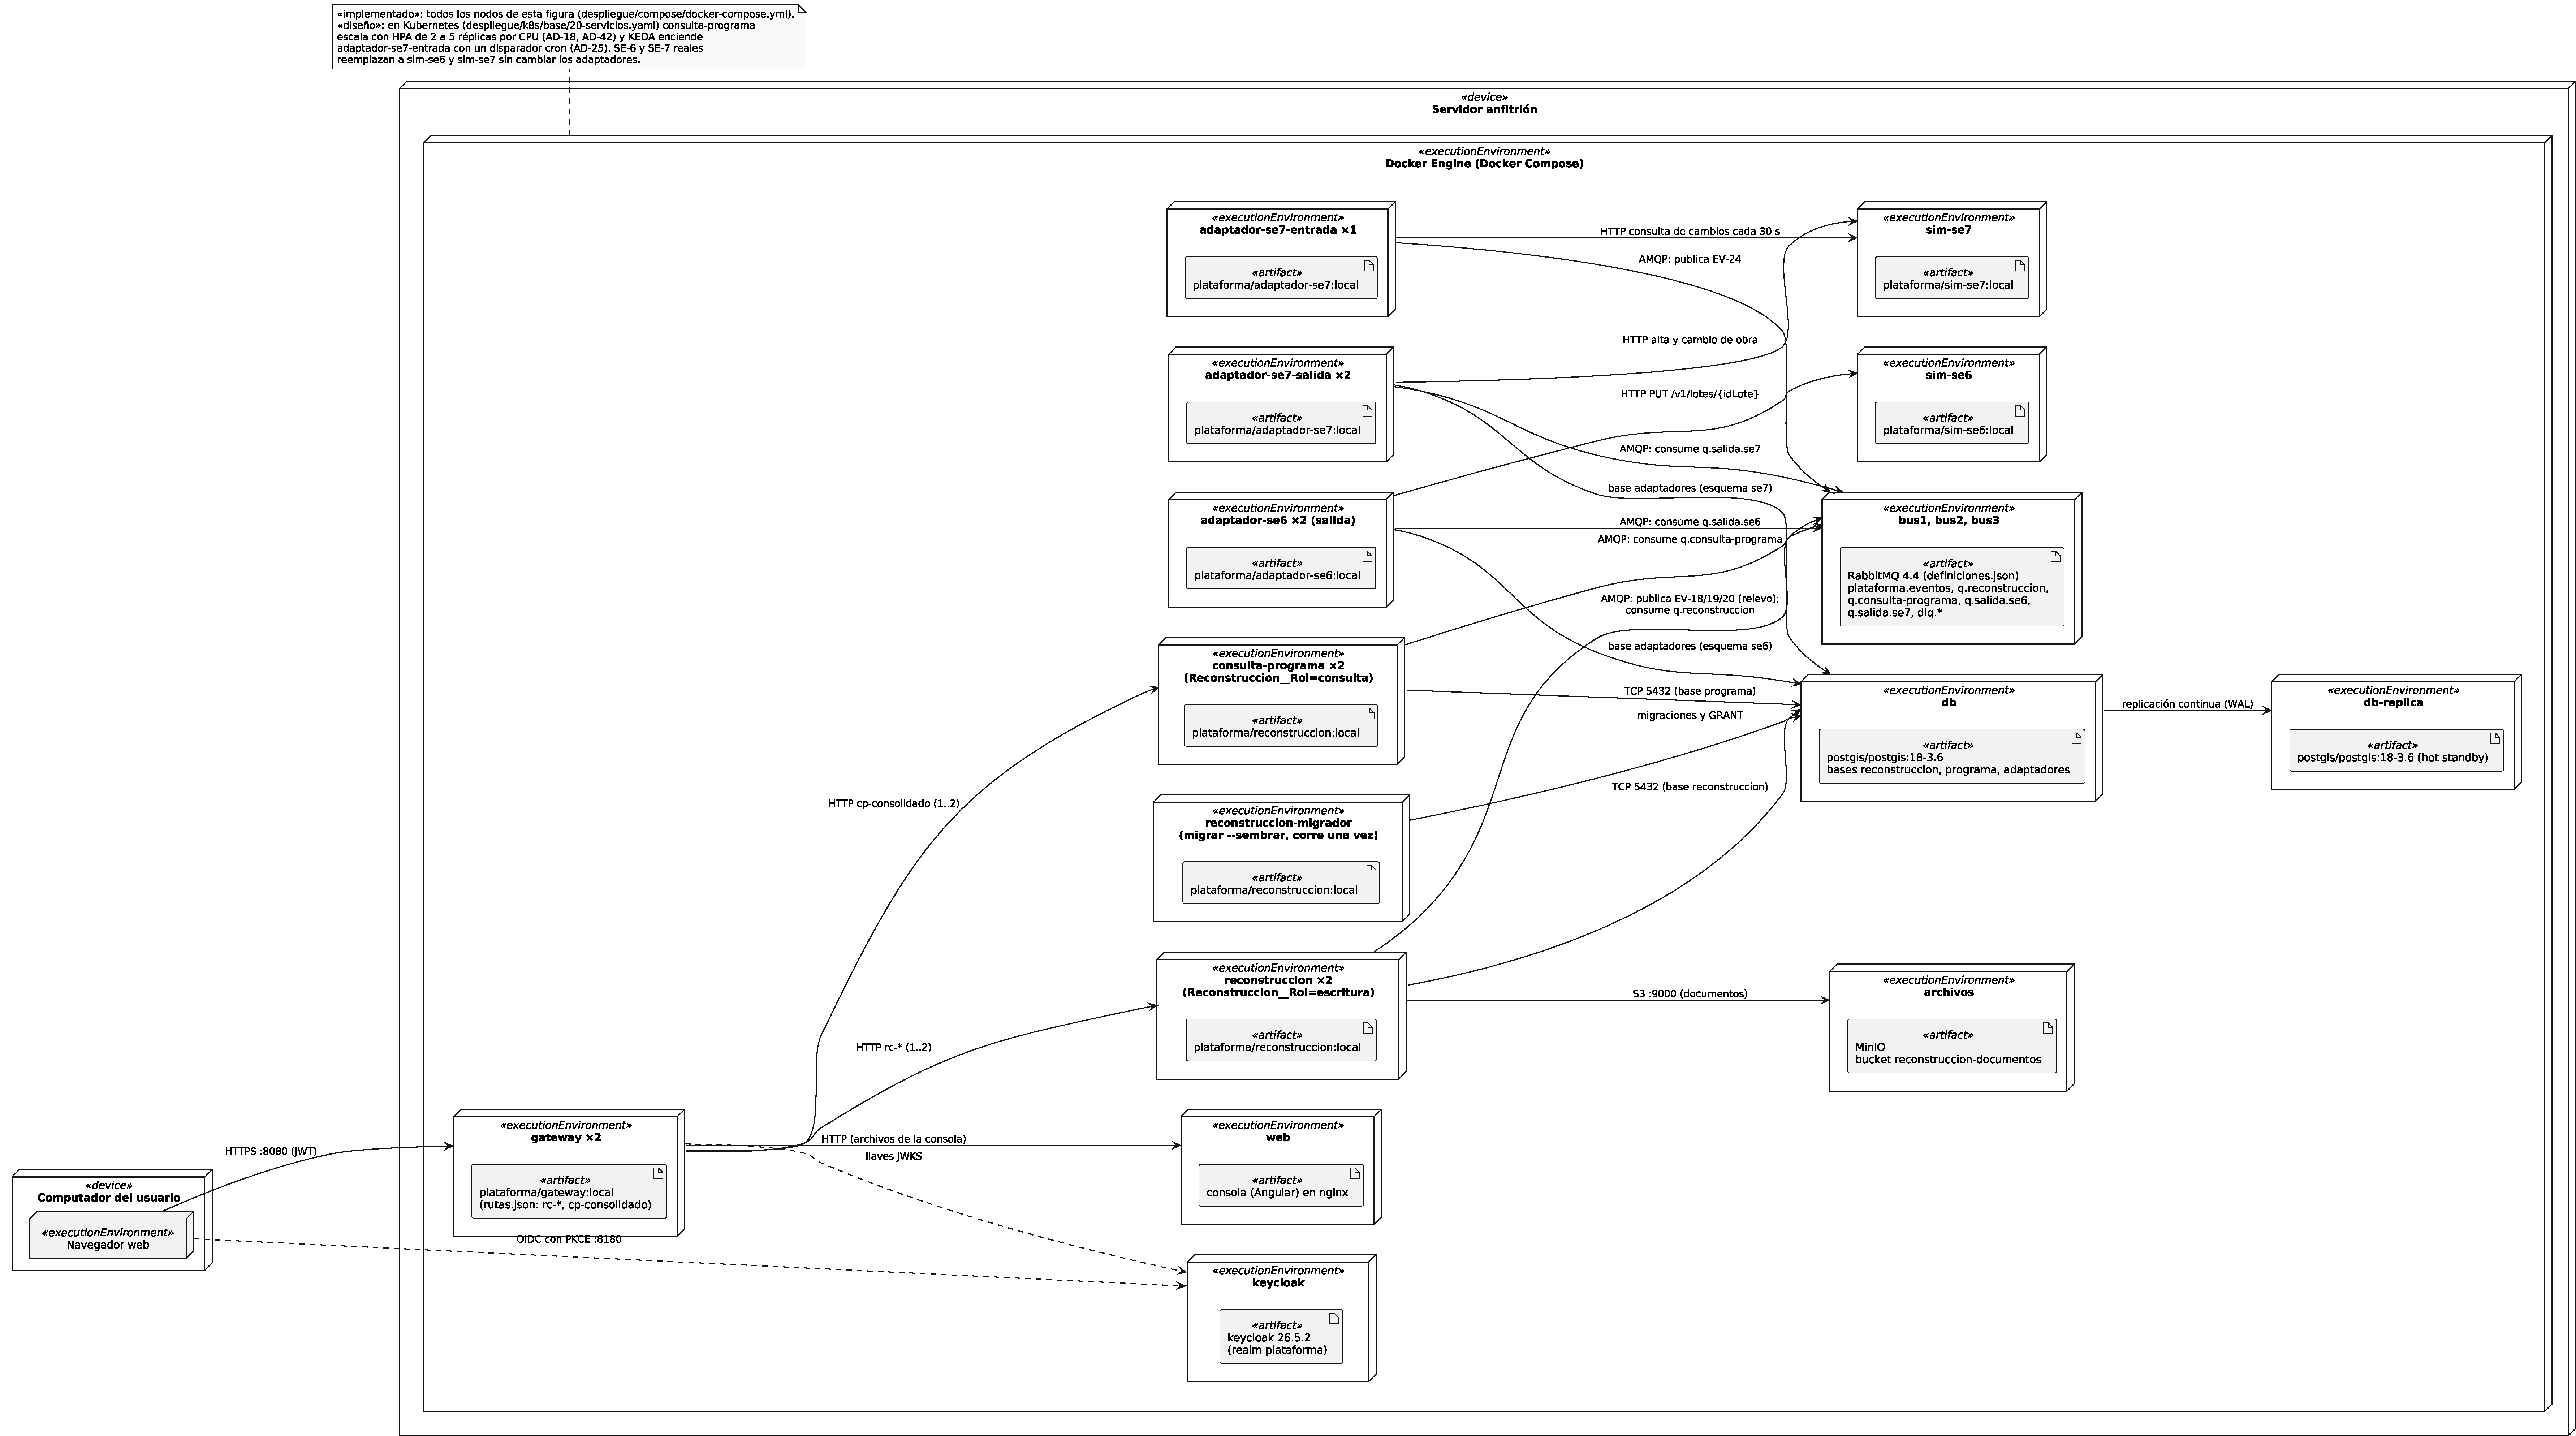
\includegraphics[width=0.88\textheight,height=\textwidth,keepaspectratio,angle=90]{08-despliegue}
  \caption{Vista física del módulo (UML de despliegue)}
  \label{fig:despliegue}
\end{figure}

\begin{itemize}
  \item \texttt{reconstruccion} corre con dos réplicas sin sesión (AD-24). Cualquier réplica atiende cualquier
        petición.
  \item \texttt{consulta-programa} es la misma imagen con \texttt{Reconstruccion\_\_Rol=consulta}, dos réplicas en
        Compose y de 2 a 5 con HPA en Kubernetes (AD-18, AD-42, AD-65).
  \item \texttt{reconstruccion-migrador} corre una vez antes de los servicios: crea los roles, aplica las migraciones
        de las bases \texttt{reconstruccion} y \texttt{programa} y siembra los datos de prueba (AD-53).
  \item \texttt{adaptador-se6} y \texttt{adaptador-se7-salida} corren con dos réplicas. \texttt{adaptador-se7-entrada}
        corre con una. Los tres entregan a los simuladores \texttt{sim-se6} y \texttt{sim-se7} (AD-25).
  \item \texttt{db} replica de forma continua en \texttt{db-replica}. \texttt{bus1}, \texttt{bus2} y \texttt{bus3}
        replican las colas quorum (AD-52, AD-54).
\end{itemize}

\clearpage
\subsection{Implementación}
\label{sec:implementacion}

La solución tiene un proyecto por anillo. Cada proyecto solo usa los que están más adentro.

{\small
\begin{longtable}{|P{4.8cm}|P{3.0cm}|P{6.8cm}|}
  \hline
  \rowcolor{cabecera}\textbf{Proyecto} & \textbf{Anillo} & \textbf{Contenido} \\ \hline
  \endfirsthead
  \hline
  \rowcolor{cabecera}\textbf{Proyecto} & \textbf{Anillo} & \textbf{Contenido} \\ \hline
  \endhead
  \texttt{Reconstruccion.\allowbreak Dominio} & Entidades & Entidades, objetos de valor, máquina de estados y jurisdicción. \\
    \hline
  \texttt{Reconstruccion.\allowbreak Aplicacion} & Casos de uso & \texttt{CasosDeUso/} (interactores), \texttt{Puertos/},
    DTO y hechos. \\ \hline
  \texttt{Reconstruccion.\allowbreak Infraestructura} & Adaptadores & \texttt{Persistencia/} (EF Core y migraciones),
    \texttt{Mensajeria/} (manejadores y bandeja), \texttt{Archivos/} (MinIO), \texttt{Registro.cs}. \\ \hline
  \texttt{Reconstruccion.\allowbreak Api} & Adaptadores & \texttt{Controllers/}, \texttt{Presenters/} y
    \texttt{Program.cs} (rol del servicio y modo migrador). \\ \hline
  \texttt{Reconstruccion.\allowbreak Pruebas} & Fuera de los anillos & Pruebas del dominio, de los casos de uso, de la
    jurisdicción y de la arquitectura, sin base de datos. \\ \hline
  \texttt{Reconstruccion.\allowbreak Integracion} & Fuera de los anillos & Pruebas con PostgreSQL y el bus: persistencia,
    eventos, copias locales, identidad y jurisdicción. \\ \hline
  \texttt{comun} (\texttt{Plataforma.Comun.*}) & Frameworks y drivers & Mensajería (bandeja, relevo, consumidor),
    eventos (\texttt{CatalogoEventos}), seguridad, migraciones y salud. \\ \hline
  \texttt{consola} (\texttt{modulos/reconstruccion}) & Frameworks y drivers & Páginas Angular del módulo. \\ \hline
\end{longtable}
}

\subsection{Alcance de la implementación y ejecución}

La implementación cubre los doce casos de uso del módulo y se integra con el resto de la plataforma:

\begin{itemize}
  \item Todo el tráfico entra por el \texttt{gateway}, que valida el token de \texttt{keycloak} y el rol de cada
        ruta. El servicio vuelve a validar el token y aplica la jurisdicción (AD-49, E-39).
  \item Las copias locales se alimentan por eventos de \texttt{gestion-desastres}, \texttt{evaluacion-danos} y
        \texttt{adaptador-se2}, sin siembra manual (AD-46).
  \item SE-6 y SE-7 se reemplazan por los simuladores \texttt{sim-se6} y \texttt{sim-se7}, que admiten modos de
        caída y lentitud para verificar QA-01.
  \item La segunda ubicación de PostgreSQL se simula con \texttt{db-replica} en el mismo anfitrión (L-01).
\end{itemize}

Para desplegar se necesita Docker. Desde la raíz del repositorio \texttt{proyectoparte2}:

\begin{verbatim}
docker compose -f despliegue/compose/docker-compose.yml up -d --build
bash pruebas/humo/prueba-humo.sh
\end{verbatim}

La consola queda en \texttt{http://localhost:8080} a través del \texttt{gateway}. Keycloak queda en
\texttt{http://localhost:8180}. La prueba de humo recorre el escenario completo: el desastre nace en Gestión de
Desastres, la evaluación se valida en Evaluación de Daños, Reconstrucción la recibe por eventos, el proyecto recorre
su ciclo y al final el desastre se puede cerrar (E-07).

% ---------------------------------------------------------------------------
\section*{Glosario}

{\small
\begin{longtable}{|P{3.4cm}|P{11.2cm}|}
  \hline
  \rowcolor{cabecera}\textbf{Término} & \textbf{Significado} \\ \hline
  \endhead
  Bandeja de salida & Tabla \texttt{bandeja\_salida} donde se guardan los eventos en la misma transacción del cambio
    (AD-45). \\ \hline
  Copia local & Datos de otro módulo guardados por Reconstrucción a partir de eventos (AD-46). \\ \hline
  DIVIPOLA & División político-administrativa del DANE: 5 dígitos para un municipio y 2 para un departamento. \\
    \hline
  DLQ & Cola de mensajes muertos (\texttt{dlq.*}) que aparta un mensaje que falla repetidamente (AD-02). \\ \hline
  Interactor & Clase que implementa un caso de uso y coordina entidades y puertos. \\ \hline
  Puerto & Interfaz del anillo de casos de uso con la que el caso de uso se comunica con el exterior. \\ \hline
  Relevo & Proceso \texttt{RelevoBandeja} que publica en el bus los eventos de la bandeja. \\ \hline
\end{longtable}
}

\subsection*{Series de identificadores}

{\small
\begin{longtable}{|P{2.4cm}|P{11.8cm}|}
  \hline
  \rowcolor{cabecera}\textbf{Serie} & \textbf{Qué identifica} \\ \hline
  \endfirsthead
  \hline
  \rowcolor{cabecera}\textbf{Serie} & \textbf{Qué identifica} \\ \hline
  \endhead
  \texttt{RF-XX-nn} & Requisito funcional del SRS. \texttt{XX} es el módulo: GD, ED, PA, RE, CO o RC. \\ \hline
  \texttt{RN-RC-nn} & Regla de negocio del módulo de Reconstrucción (RN-RC-01 a RN-RC-22). \\ \hline
  \texttt{QA-nn} & Escenario de atributo de calidad del SRS (QA-01 a QA-15). \\ \hline
  \texttt{FP-nn} & Caso de uso de la funcionalidad primaria del SRS (FP-01 a FP-10). \\ \hline
  \texttt{SE-n} & Familia de sistemas externos (SE-1 a SE-8). \\ \hline
  \texttt{CU-nn} & Caso de uso del módulo de Reconstrucción (CU-01 a CU-12). \\ \hline
  \texttt{AD-nn} & Decisión del SAD: AD-01 a AD-49 son estructurales y AD-50 a AD-65 son de tecnología. \\ \hline
  \texttt{DA-nn} & Decisión de la revisión de arquitectura previa a la implementación. \\ \hline
  \texttt{DM-nn} & Decisión de diseño del módulo de Reconstrucción (DM-01 a DM-11). \\ \hline
  \texttt{E-nn} & Enmienda a los documentos, surgida de la revisión y de la implementación (E-01 a E-43). \\ \hline
  \texttt{EV-nn} & Evento del catálogo del SAD (EV-01 a EV-29). \\ \hline
  \texttt{L-nn} & Límite declarado de la implementación (L-01 a L-10). \\ \hline
  \texttt{R-nn} & Riesgo del ATAM (R-01 a R-14). \\ \hline
\end{longtable}
}

\subsection*{Límites declarados de la implementación}

Provienen de la revisión de arquitectura del proyecto \cite{revision}.

{\small
\begin{longtable}{|P{1.4cm}|P{12.8cm}|}
  \hline
  \rowcolor{cabecera}\textbf{ID} & \textbf{Límite} \\ \hline
  \endfirsthead
  \hline
  \rowcolor{cabecera}\textbf{ID} & \textbf{Límite} \\ \hline
  \endhead
  L-01 & Una sola región: no hay enrutador global ni réplica en otra ubicación (AD-26, AD-27, QA-03). \\ \hline
  L-02 & Los rechazos del punto de entrada y la alarma de la bandeja de revisión no se registran en Auditoría (QA-11, R-08). \\ \hline
  L-03 & No hay pruebas de carga en un clúster ni de caos (QA-05, QA-06 y la consulta de 10\,000 entradas de QA-13). \\ \hline
  L-04 & Las latencias se midieron con 20 clientes en un computador, no con 10\,000 usuarios. \\ \hline
  L-05 & El despliegue en el clúster local no se verificó de punta a punta, y el inicio de sesión exige reenviar puertos. \\ \hline
  L-06 & Fuera de la implementación: Consolidación, Notificación (SE-8, QA-08), Gestión de Recursos, Personas Afectadas (QA-12), Coordinación de Organismos, Portal público y adaptadores de SE-1, SE-3, SE-4, SE-5 y SE-8. \\ \hline
  L-07 & La aplicación móvil entregada es la variante de depuración, que admite conexiones sin cifrar, y el proveedor de identidad corre sin TLS. \\ \hline
  L-08 & El emisor de los tokens es una dirección local: el emulador necesita reenviar ese puerto y un teléfono físico exige cambiar la dirección en el proveedor y en quienes validan el token. \\ \hline
  L-09 & Pendientes menores: filtro de Auditoría por jurisdicción, validación condicional en la descarga, aviso de activo fusionado al cliente incremental, base única del adaptador de SE-2, índice del historial por municipio, recarga de las llaves del token y evaluaciones rechazadas en la consola. \\ \hline
  L-10 & La aplicación móvil adjunta solo fotografías como evidencia, y la evidencia no guarda un autor propio (RF-ED-03 parcial). \\ \hline
\end{longtable}
}

\subsection*{Enmiendas citadas en este documento}

{\small
\begin{longtable}{|P{1.4cm}|P{12.8cm}|}
  \hline
  \rowcolor{cabecera}\textbf{ID} & \textbf{Enmienda} \\ \hline
  \endfirsthead
  \hline
  \rowcolor{cabecera}\textbf{ID} & \textbf{Enmienda} \\ \hline
  \endhead
  E-01 & Reconstrucción consume EV-08 y obtiene las candidatas de su copia local, sin consultar a Consulta de Daños (AD-46). \\ \hline
  E-04 & Evento nuevo EV-24: avance o contratista reportado por SE-7. \\ \hline
  E-07 & Gestión de Desastres consume EV-18 y EV-20: un desastre no se cierra con proyectos no finales (AD-47). \\ \hline
  E-09 & Rutas que faltaban en el catálogo de APIs. \\ \hline
  E-10 & Contenido de EV-18, EV-19 y EV-20: EV-19 lleva presupuesto y fuente, y EV-20 lleva cronograma, responsable, avance y costo. \\ \hline
  E-19 & La bandeja de salida se aplica en todo microservicio productor (AD-45). \\ \hline
  E-20 & Jurisdicción de la aprobación: autoridad local, regional o nacional según el territorio del proyecto. \\ \hline
  E-28 & Origen de las candidatas en el diseño de Reconstrucción: copia local alimentada por eventos. \\ \hline
  E-36 & Reconstrucción consume EV-21 para mostrar el nombre del municipio. \\ \hline
  E-39 & La autoridad solo ve y usa los proyectos y las evaluaciones de su jurisdicción. \\ \hline
\end{longtable}
}

\begin{thebibliography}{99}

\bibitem{enunciado}
Departamento de Ingeniería de Sistemas, Pontificia Universidad Javeriana. \textit{Arquitectura de
Software. Proyecto del semestre: Plataforma para la Gestión de Desastres y Reconstrucción}.
Enunciado, versión 0.9, 2026.

\bibitem{srs}
S. Gantiva, D. Guiza y J. Rubiano. \textit{Especificación de Requisitos de Software (SRS). Plataforma para la Gestión
de Desastres y Reconstrucción}. Versión 1.2, 18 de noviembre de 2026.

\bibitem{sad}
S. Gantiva, D. Guiza y J. Rubiano. \textit{Documento de Arquitectura de Software (SAD). Plataforma para la Gestión de
Desastres y Reconstrucción}. Versión 1.2, 18 de noviembre de 2026.

\bibitem{atam}
S. Gantiva, D. Guiza y J. Rubiano. \textit{Evaluación de la arquitectura mediante ATAM. Plataforma para la Gestión de
Desastres y Reconstrucción}. Versión 1.2, 18 de noviembre de 2026.

\bibitem{revision}
S. Gantiva, D. Guiza y J. Rubiano. \textit{Revisión de arquitectura y plan de integración} y \textit{Enmiendas
propuestas a los documentos}. Repositorio \texttt{proyectoparte2}, rama \texttt{cierre-implementacion}, 18 de noviembre
de 2026.

\bibitem{bass}
L. Bass, P. Clements y R. Kazman. \textit{Software Architecture in Practice}. 4.ª edición.
Addison-Wesley, 2021.

\bibitem{iso25010}
ISO/IEC 25010:2011. \textit{Systems and software engineering. Systems and software Quality
Requirements and Evaluation (SQuaRE). System and software quality models}. International
Organization for Standardization, 2011.

\bibitem{iso42010}
ISO/IEC/IEEE 42010:2011. \textit{Systems and software engineering. Architecture description}.
International Organization for Standardization, 2011.

\bibitem{clements}
P. Clements, F. Bachmann, L. Bass, D. Garlan, J. Ivers, R. Little, P. Merson, R. Nord y J. Stafford.
\textit{Documenting Software Architectures: Views and Beyond}. 2.ª edición. Addison-Wesley, 2011.

\bibitem{kruchten}
P. Kruchten. \textit{Architectural Blueprints: The ``4+1'' View Model of Software
Architecture}. IEEE Software, 12(6), 1995.

\bibitem{martin}
R. C. Martin. \textit{Clean Architecture: A Craftsman's Guide to Software Structure and Design}.
Prentice Hall, 2017.

\end{thebibliography}

\end{document}
